% Fundamentals of Microcontrollers Manual
% 
% Manual to accompany the class lectures and lab
%
% Seth McNeill
% Started 2021 November 16

\documentclass[12pt,oneside]{book}
\usepackage{datetime}  % for automated current date on the document
\setcounter{secnumdepth}{3}  % to make subsubsections numbered
\usepackage{amsmath}  % for aligned equations and such
\usepackage[table]{xcolor}  % to color text
\usepackage[pdftex]{graphicx} % for includegraphics?
\usepackage{siunitx}  % for aligning tables by decimal point
\usepackage{pdfpages}  % to include PDF files in the document
\usepackage{listings}  % for code listings

% For creating nice addition figures
% based on https://tex.stackexchange.com/a/96764
\usepackage{cancel}
\usepackage{physics}  % for derivative symbols
\usepackage{tikz}
\usetikzlibrary{matrix, shapes, arrows.meta, positioning, angles, quotes}
\newcommand{\addend}{\text{\textsl{\color{gray}{Addend}}}}
\newcommand{\augend}{\text{\textsl{\color{gray}{Augend}}}}
\newcommand{\sumOut}{\text{\textsl{\color{gray}{Sum}}}}
% end addition figure requirements
\usepackage{hyperref}  % for URL hyperlinks

\hypersetup{
colorlinks,
citecolor=black,
filecolor=black,
linkcolor=blue,
urlcolor=blue
}

% setup listings for C++ and desired results
\lstset{ %
  backgroundcolor=\color{white},   % choose the background color; you must add \usepackage{color} or \usepackage{xcolor}
  basicstyle=\fontfamily{pcr}\selectfont,        % the size of the fonts that are   basicstyle=\fontfamily{psc}\selectfont,        % the size of the fonts that are used for the code
  breakatwhitespace=false,         % sets if automatic breaks should only happen at whitespace
  breaklines=true,                 % sets automatic line breaking
  captionpos=b,                    % sets the caption-position to bottom
%  commentstyle=\color{green},    % comment style
  escapeinside={\%*}{*)},          % if you want to add LaTeX within your code
  keepspaces=true,                 % keeps spaces in text, useful for keeping indentation of code (possibly needs columns=flexible)
  keywordstyle=\color{blue},       % keyword style
  language=C++,                 % the language of the code
  numbers=none,                    % where to put the line-numbers; possible values are (none, left, right)
  rulecolor=\color{black},         % if not set, the frame-color may be changed on line-breaks within not-black text (e.g. comments (green here))
  showspaces=false,                % show spaces everywhere adding particular underscores; it overrides 'showstringspaces'
  showstringspaces=false,          % underline spaces within strings only
  showtabs=false,                  % show tabs within strings adding particular underscores
  stringstyle=\color{black},     % string literal style
  tabsize=2,                       % sets default tabsize to 2 spaces
  title=\lstname                   % show the filename of files included with \lstinputlisting; also try caption instead of title
}


% for automated current date on the document
\newdateformat{myDate}{\THEYEAR{ }\monthname[\THEMONTH] \twodigit{\THEDAY}}

% Referencing commands 
\newcommand{\chaplabel}[1]{\label{chap:#1}}
\newcommand{\chapref}[1]{Chapter~\ref{chap:#1}}
\newcommand{\seclabel}[1]{\label{sec:#1}}
\newcommand{\secref}[1]{Section~\ref{sec:#1}}

\title{Fundamentals of Applied Microcontrollers Manual}
\author{Seth McNeill}
\date{Edition 0.01 \\ \myDate\today}

\begin{document}
	\maketitle

	\tableofcontents

	% include chapters here
	\chapter{Introduction}
\chaplabel{intro}

This book is the accompanying text to a class introducing Microcontrollers
to upper division, non-electrical engineering undergraduate students who 
have taken some C programming.
	\chapter{Number Systems}
\chaplabel{numbers}

This chapter introduces the concepts of different numbering systems that
are relevant to microcontrollers.

\section{Decimal Numbers}
The standard number system used by humans is based on 10. This logically flows 
the usual numbers of fingers or toes humans have. When counting in the base 10 (decimal) we 
start at 0, count up to 9, then run out of numbers 
to use. When runs out of numbers, we put a number to the left of the column we were counting
in, and then start over at zero again which gives us the number 10. A more clear way to count 
would be to count from 00 to 09, then increment the left digit and start the right digit back
at 0. This can be continued until 99 is reached. But now we have a model to follow. If a 
column gets to 9, we increment a column to the left and start the current column over at 0. 
This leads to the number 100. This concept can be continued forever.

When given a particular number, 3254, in decimal the value is calculated as
\begin{equation}
	3254 = 3\cdot1000 + 2\cdot100 + 5\cdot10 + 4
\end{equation}
It could also be represented as
\begin{equation}
	3254 = 3\cdot10^3 + 2\cdot10^2 + 5\cdot10^1 + 4\cdot10^0
\end{equation}
This is the basis for a positional number system.

\section{Binary Numbers}
Computers run a base 2 system, also known as binary. This means that we only have two options 
at each position, 1 or 0, instead of the 10 available in the decimal system. However, counting
is done in the same way, when you run out of symbols, increment the position to the left and 
then start over at zero in the current position.

Binary numbers are also positional so a number like 1011 is 
\begin{equation}
	1011 = 1\cdot2^3 + 0\cdot2^2 + 1\cdot2^1 + 1\cdot2^0 = 11_{10}
\end{equation}
where $11_{10}$ indicates that the number 11 is base 10.

The maximum value a binary number can have is determined by the number of bits it has. The formula is: 
\begin{equation}
	V_{max} = 2^n - 1
\end{equation}
where n is the number of bits. For example, an 8 bit number has a maximum value of $2^8 - 1 = 255$.

\section{Hexadecimal Numbers}
\begin{sloppypar}
The problem for humans is that we have a very difficult time reading binary numbers. Especially once the
numbers get long such as $11101101010010110101_2$. The first thing we can do to improve intelligibility is to 
put a space in every 4 digits so that we aren't completely bowled over by all the digits. This gives us
$1110~1101~0100~1011~0101_2$. This is better but still leaves some challenges. Someone pointed out that since
4~bits can have 16 different values, what if each 4~bits (also called a nibble) was represented by a single
base 16 number. Base 16 is called hexadecimal. It has the problem that it runs out of digits once we get to 
10, so it was decided to simply start on the alphabet so $10_{10}$ is $A_{16}$, $11_{10}$ is $B_{16}$, and so forth. Now 
the cumbersome binary number we've been playing with can be represented as $ED4B5_{16}$. 
\end{sloppypar}

A comparison of the different numbering system representations of 0 through $15_{10}$ are shown in 
Table~\ref{table:numsystems}.

\begin{table}[!ht]
	\centering
	\begin{tabular}{c c c}
		\hline
		Decimal & Binary & Hexadecimal \\ 
		\hline
		00 & 0000 & 0 \\
		01 & 0001 & 1 \\
		02 & 0010 & 2 \\
		03 & 0011 & 3 \\
		04 & 0100 & 4 \\
		05 & 0101 & 5 \\
		06 & 0110 & 6 \\
		07 & 0111 & 7 \\
		08 & 1000 & 8 \\
		09 & 1001 & 9 \\
		10 & 1010 & A \\
		11 & 1011 & B \\
		12 & 1100 & C \\
		13 & 1101 & D \\
		14 & 1110 & E \\
		15 & 1111 & F \\
		\hline
	\end{tabular}
	\caption{Decimal, binary, and hexadecimal numbers align as shown in this table.}
	\label{table:numsystems}
\end{table}

\section{Binary Background}
The reasons for this stem from early computers 
using switches (relays) as their basic computing elements and the fact that telling the 
difference between a ``high" voltage and a ``low" voltage is easier to do than to differentiate
10 different voltages. It also allows for a gap between high and low that creates some 
immunity to noise called the \href{https://3.bp.blogspot.com/-7GOaQqAncoU/VelAErlx5gI/AAAAAAAARLE/kITWaG8LAws/s1600/noise%2Bmargin.png}{noise margin}. 
The figure linked to labels noise margin at NM which indicates how much (in volts) the signal coming
from the source on the left can be degraded and still be recognized as a high or low. The other 
cool thing about digital signals is that each device the signal passes through removes
all noise.

\section{Converting Between Bases}
\subsection{Binary to Decimal}
Converting to decimal is straightforward since we can simply sum each digit multiplied by the 
power of 2 it represents. 
\begin{equation}
	\label{eq:bin2dec}
	V_{10} = \sum_{i=0}^p d_i \cdot 2^i
\end{equation}
In Equation~\ref{eq:bin2dec} the $p$ digits, $d_i$, of the binary number are summed from right 
to left while being multiplied by the power of 2 they represent. As an example, convert 
1011~0111 to decimal.
\begin{equation}
	\begin{split}
	V_{10} &= 1\cdot2^0 + 1\cdot2^1 + 1\cdot2^2 + 0\cdot2^3 + 1\cdot2^4 + 1\cdot2^5 + 0\cdot2^6 + 1\cdot2^7\\
		&= 1 + 2 + 4 + 0 + 16 + 32 + 0 + 128\\
		&= 183
	\end{split}
\end{equation}
I usually find it easiest to just remember the powers of two for each place and add them up.
\begin{equation}
	\overset{128}{1}\quad\overset{64}{0}\quad\overset{32}{1}\quad\overset{16}{1}\quad\overset{8}{0}\quad
	\overset{4}{1}\quad\overset{2}{1}\quad\overset{1}{1} = 1 + 2 + 4 + 16 + 32 + 128
\end{equation}

\subsection{Decimal to Binary}
Converting decimal numbers to binary involves dividing by 2 until the remainder is 0 or 1. The process
goes as follows:
\begin{enumerate}
	\item  Divide the number by 2. If the remainder is 1 then the least significant bit is 1 otherwise if the remainder is 0 
	(it was an even number) then the least significant bit is 0.
	\item \label{st:d2b2}Take the quotient from the previous step and divide by 2. The remainder is the next more significant bit in the binary representation.
	\item Repeat Step \ref{st:d2b2} until the quotient is 0.
\end{enumerate}

As an example, let's convert $11_{10}$ to binary. 
\begin{equation}
	\begin{aligned}
		11 \divisionsymbol 2 & = 5R1 &\rightarrow 1 &\mathrm{~(LSB)} \\
		5 \divisionsymbol 2 & = 2R1 &\rightarrow 1 \\
		2 \divisionsymbol 2 & = 1R0 &\rightarrow 0 \\
		1 \divisionsymbol 2 & = 0R1 &\rightarrow 1 & \mathrm{~(MSB)}
	\end{aligned}
\end{equation}
That means that $11_{10}$ is $1011_2$. As another example let us convert $20_{10}$ to binary.
\begin{equation}
	\begin{aligned}
		20 \divisionsymbol 2 & = 10R0 &\rightarrow 0 &\mathrm{~(LSB)}\\
		10 \divisionsymbol 2 & = 5R0  &\rightarrow 0 \\
		5 \divisionsymbol 2 &  = 2R1  &\rightarrow 1 \\
		2 \divisionsymbol 2 &  = 1R0  &\rightarrow 0 \\
		1 \divisionsymbol 2 &  = 0R1  &\rightarrow 1 & \mathrm{~(MSB)}
	\end{aligned}
\end{equation}
This shows that $20_{10}$ is $10100_2$.

\subsection{Binary and Hexadecimal}
For conversions between binary and hexadecimal I tend to use the table lookup method. After using it 
enough times you begin to memorize the conversions. In my head I'm usually converting from binary to 
decimal on each nibble and then converting decimal into hexadecimal. So if I see 0101 I remember it 
is 5 in decimal which is the same in hex. If I see 1010 I remember that it is $8 + 2 = 10$ which is 
one more than 9 so it is A in hex.

\section{Colors}
Colors for display on computers are represented as binary numbers. Colors are 24~bit which is broken
down into 3 8~bit numbers representing red, green, and blue (RGB). Eight bits give values over the 
range of 0 to 255 so colors are represented by 3 numbers such as (255, 0, 255) which gives a 
\textcolor[RGB]{255, 0, 255}{color like this}. It is good to note that (255, 255, 255) is white,
(0, 0, 0) is black, and (X, X, X) where all three numbers are the same is gray.

Sometimes colors are represented as a 6~digit binary number in hexadecimal form prefixed by 0x such 
as 0xFF00FF for the color we looked at previously. 

\section{ASCII}
Since computers operate using binary numbers, how do we get them to represent human languages? The method 
caught it is called \href{https://en.wikipedia.org/wiki/ASCII}{American Standard Code for Information Interchange (ASCII)}. Basically, 7~bit numbers
were mapped to letters, numbers, punctuation, symbols, and control characters. Some examples are A is 65, Z 
is 90, a is 97, z is 122, 0 is 48, 9 is 57. The most used control characters are carriage return (13 or \textbackslash r) and 
line feed (10 or \textbackslash n). Unix based operating systems (Linux, OS X) use line feed to indicate a new line. Windows
uses both (\textbackslash r\textbackslash n).

Look up an ASCII table online when you need to know the values.

\section{Adding and Subtracting Binary Numbers}
\subsection{Default method}

\subsubsection{Addition}
% addition method based on https://tex.stackexchange.com/a/96764
Calculate the binary sum $0001\;0011\;1101+0000\;1011\;0111$.
\begin{equation}
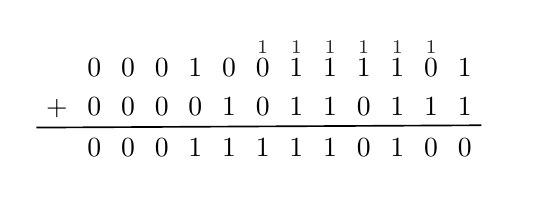
\begin{tikzpicture}[
    row 1/.style={font=\textsl,font=\scriptsize,black!85, %anchor=west,
        inner sep=1.5pt, row sep=-3pt},
    every node/.style={column sep=.5pt,row sep=1pt}]
    \matrix (m) [matrix of math nodes,
        nodes in empty cells,
        %nodes=draw
    ] 
    {
        &   &   &   &   &   & 1 & 1 & 1 & 1 & 1 & 1 &   &                   \\
        & 0 & 0 & 0 & 1 & 0 & 0 & 1 & 1 & 1 & 1 & 0 & 1 &[10mm] \\
    +   & 0 & 0 & 0 & 0 & 1 & 0 & 1 & 1 & 0 & 1 & 1 & 1 &  \\ 
        & 0 & 0 & 0 & 1 & 1 & 1 & 1 & 1 & 0 & 1 & 0 & 0 &  \\                                                  
    };

    \draw[-,color=black,semithick] (m-3-1.south west) -- (m-3-13.south east);

\end{tikzpicture}
\label{binary_integer_addition}
\end{equation}

\subsubsection{Subtraction}
Calculate the binary difference $0001\;0011\;1101-0000\;1011\;0111$.
\begin{equation}
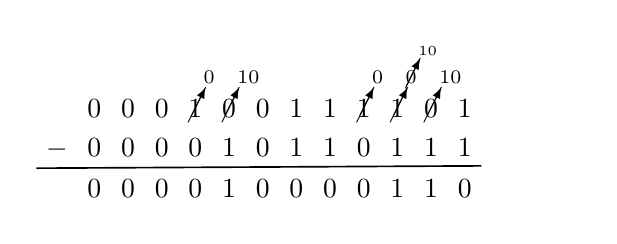
\begin{tikzpicture}[
    every node/.style={column sep=.5pt,row sep=1pt}]
    \matrix (m) [matrix of math nodes,
        nodes in empty cells,
        %nodes=draw
    ] 
    {
        & 0 & 0 & 0 & \cancelto{0}{1} & \cancelto{10}{0} & 0 & 1 & 1 & \cancelto{0}{1} & \cancelto{\cancelto{10}{0}}{1} & \cancelto{10}{0} & 1 &[10mm] \\
    -   & 0 & 0 & 0 & 0 & 1 & 0 & 1 & 1 & 0 & 1 & 1 & 1 &  \\ 
        & 0 & 0 & 0 & 0 & 1 & 0 & 0 & 0 & 0 & 1 & 1 & 0 &  \\                                                  
    };

    \draw[-,color=black,semithick] (m-2-1.south west) -- (m-2-13.south east);

\end{tikzpicture}
\label{binary_integer_subraction}
\end{equation}


\subsection{Twos Complement method}

\begin{table}[!ht]
	\centering
	\begin{tabular}{S c}
		\hline
		{Decimal} & {Two's Complement} \\ 
		\hline
		7 & 0111 \\
		6 & 0110 \\
		5 & 0101 \\
		4 & 0100 \\
		3 & 0011 \\
		2 & 0010 \\
		1 & 0001 \\
		0 & 0000 \\
		-1 & 1111 \\
		-2 & 1110 \\
		-3 & 1101 \\
		-4 & 1100 \\
		-5 & 1011 \\
		-6 & 1010 \\
		-7 & 1001 \\
		-8 & 1000 \\
		\hline
	\end{tabular}
	\caption{This table shows the decimal and two's complement numbers for 4-bits.}
	\label{table:twoscomplement}
\end{table}


\section{Gray Codes}
When counting in binary, often times more than one bit changes as the number increments. This works fine
in the ideal world, but in the real world, the logic controlling each bit might be slightly different. This 
will cause one bit to change at a slightly different time than another bit. That causes glitches in the counting
that can be disruptive to the overall system. 

Take as an example a robot that represents the cardinal directions as binary integers as illustrated in Figure \ref{fig:nongraydir}.
\begin{figure}[!htb]
	\centering
	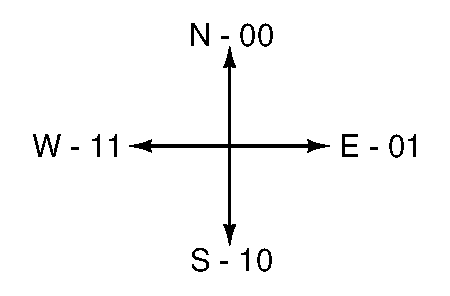
\includegraphics[scale=0.7]{numbers/nongray.eps}
	\caption{This figure shows using regular binary counting to represent the cardinal directions.}
	\label{fig:nongraydir}
\end{figure} 

Using regular binary counting means that as the direction changes from East to South, two bits have to change. If the bits
are driven by real switches or differing logic they may not change simultaneously leading to possible outputs
of E~-~W~-~S or E~-~N~-~S. If the data is being used in a sequential manner it could lead to erroneous actions by
the device (robot, car, etc.). Instead of using regular binary counting, we could use an encoding that only changes
one bit at a time as the directions change as shown in Figure \ref{fig:graydir}.
\begin{figure}[!htb]
	\centering
	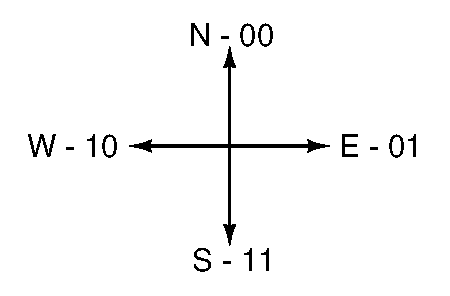
\includegraphics[scale=0.7]{numbers/gray.eps}
	\caption{This figure shows using Gray codes to represent the cardinal directions.}
	\label{fig:graydir}
\end{figure} 

Counting systems like this are called Gray code after \href{https://en.wikipedia.org/wiki/Gray_code}{Frank Gray} 
or reflected binary code. A 4-bit example is shown in Table \ref{table:graycode}.

\begin{table}[!ht]
	\centering
	\begin{tabular}{c}
		\hline
		{Gray Code}   \\ 
		\hline
		0000 \\
		0001 \\
		0011 \\
		0010 \\
		\hline
		0110 \\
		0111 \\
		0101 \\
		0100 \\
		\hline
		1100 \\
		1101 \\
		1111 \\
		1110 \\
		1010 \\
		1011 \\
		1001 \\
		1000 \\
		\hline
	\end{tabular}
	\caption{This table shows 4-bit Gray codes with horizontal lines showing the break for 2- and 3-bit Gray codes.}
	\label{table:graycode}
\end{table}

\section{Binary Background}
Originally, computers were just a bunch of switches, therefore, they only had two positions: on and off. 
This also has the benefit that there is a large amount of noise immunity. A repeater (buffer) can eliminate 
by recreating the original signal without noise. These are all great benefits of the binary system.

	\chapter{Boolean Logic}
\chaplabel{logic}

\section{Introduction}
This chapter introduces some basic Boolean logic including gates and Boolean algebra.

When can you drive through an intersection? When the light is NOT red. This is the first and simplest
logic operator--the NOT element. It simply changes any TRUE to FALSE or FALSE to TRUE (you can substitute
1 for TRUE and 0 for FALSE, or on/off).

Another way to think about stop lights is that it is legal to go through the intersection 
if the light is green OR yellow. Or you must stop if the light is NOT green AND NOT yellow. 
Let's build a table of values for each of these situations. 

\begin{table}[!ht]
	\centering
	\begin{tabular}{| c | c |}
		\hline
		\textbf{RED} & \textbf{GO} \\ 
		\hline
		TRUE & FALSE  \\ \hline
		FALSE & TRUE  \\ \hline
	\end{tabular}
	\caption{Legally driving through an intersection can be written using a NOT function.}
	\label{table:stoptf}
\end{table}

\begin{table}[!ht]
	\centering
	\begin{tabular}{| c | c |}
		\hline
		\textbf{RED} & \textbf{GO} \\ 
		\hline
		1 & 0  \\ \hline
		0 & 1  \\ \hline
	\end{tabular}
	\caption{Crossing an intersection can also be done with 0/1 rather than TRUE/FALSE.}
	\label{table:stop01}
\end{table}

\begin{table}[!ht]
	\centering
	\begin{tabular}{| c | c | c |}
		\hline
		\textbf{GREEN} & \textbf{YELLOW} & \textbf{GO} \\ 
		\hline
		FALSE & FALSE & FALSE \\ \hline
		FALSE & TRUE  & TRUE  \\ \hline
		TRUE  & FALSE & TRUE  \\ \hline
		\sout{TRUE}  & \sout{TRUE}  & \sout{TRUE}  \\ \hline
	\end{tabular}
	\caption{Legally driving through an intersection can be written using an OR function.
                Note that normally in the US, the green and yellow lights should not both be on.}
	\label{table:stopor}
\end{table}

How do you start a car? In most of the cars I have driven I have to press on the brake at the 
same time as I turn the key. To say it another way, the car starts when I press the break
AND turn the key.
\begin{equation}
	pressBreak \: \mathrm{AND} \: turnKey = startedCar
\end{equation}
Again on a car, a particular blinker light will turn on if you turn on the turn signal or if you turn on the 4-way blinker.
\begin{equation}
	turnSignal \: \mathrm{OR} \: 4wayBlinker = blinking
\end{equation}
The AND and OR in the equation are Boolean operators. 

\section{Methods of Representing Logic}
It is important to differentiate between different forms of representation because $\overline{\mathrm{EN}}$
means \textbf{active low} enable. It does not mean NOT(E AND N). The understanding of which method is being 
used is usually derived from context. Using the dot ($\cdot$) everywhere can become burdensome, so when context
makes it obvious (usually examples involving A, B, and C or X and Y) we may drop the dots and just use adjacency to represent
the AND function.

In this class, most of the logic you write will be done in C++. Some of the following tables will also
address how to represent logic in C++.

Going back to the stoplight example, we can look at the same information using the nomenclature just 
introduced.
\begin{subequations}
    \begin{align}
    GO &= \overline{RED} \\
    GO &= GREEN + YELLOW \\
    STOP &= \overline{GREEN}\cdot\overline{YELLOW} \\
    \overline{GO} &= \overline{GREEN}\cdot\overline{YELLOW}
    \end{align}
\end{subequations}

\section{Boolean Algebra}

\subsection{Theorems of Boolean Algebra}
Ways to show NOT:
\begin{subequations}
	\begin{alignat}{3}
        &\mathrm{Algebra} &&\quad \mathrm{C++}\notag \\
	NOT(X) &= \overline{X} = X^{\prime} &&\quad !x \\
	\overline{(\overline{X})} &= \left(X^{\prime}\right)^{\prime}= X &&\quad !(!x) = x
	\end{alignat}
\end{subequations}
Rules of AND and OR:
\begin{subequations}
	\begin{align}
	\mathrm{AND} \quad & \mathrm{OR}\notag\\
	0\cdot0 = 0 \quad & 1+1 = 1\\
	1\cdot1 = 1 \quad & 0+0 = 0\\
	0\cdot1 = 1\cdot0 = 0 \quad & 1 + 0 = 0 + 1 = 1
	\end{align}
\end{subequations}
And repeated in C++ form:
\begin{subequations}
    \begin{align}
	\mathrm{AND} \quad & \mathrm{OR}\notag\\
	\mathrm{false\: \&\&\: false == false} \quad & \mathrm{true\:||\:true\:==\:true}\\
	\mathrm{true\: \&\&\: true == true} \quad & \mathrm{false\:||\:false\:==\:false}\\
	\mathrm{true\: \&\&\: false == false} \quad & \mathrm{true\:||\:false\:==\:true}
    \end{align}
\end{subequations}

\begin{subequations}
	\begin{align}
	\mathrm{AND} \qquad & \mathrm{OR}\notag\\
	X\cdot1 = X \qquad & X + 0 = X\\	
	X\cdot0 = 0 \qquad & X + 1 = 1\\	
	X\cdot X = X \qquad & X + X = X\\	
	X\cdot\overline{X} = 0 \qquad & X + \overline{X} = 1
	\end{align}
\end{subequations}

For two and three variables you have the following useful equations:
\begin{subequations}
	\begin{align}
	\mathrm{AND} \qquad & \mathrm{OR}\notag \\
	X\cdot Y = Y \cdot X \qquad & X + Y = Y + X \\
	(X \cdot Y) \cdot Z = X \cdot (Y \cdot Z) \qquad & (X + Y) + Z = X + (Y + Z) \\
	(X + Y)\cdot (X + Z) = X + Y\cdot Z \qquad & X\cdot Y + X\cdot Z = X\cdot (Y + Z) \\
	X\cdot (X + Y) = X \qquad & X + X\cdot Y = X \\
	(X + Y) \cdot (X + \overline{Y}) = X \qquad & X\cdot Y + X\cdot \overline{Y} = X \\
	X\cdot (\overline{X} + Y) = X\cdot Y \qquad & X + \overline{X} \cdot Y = X + Y
	\end{align}
	\begin{equation}
	X\cdot Y + \overline{X}\cdot Z + Y\cdot Z = X\cdot Y + \overline{X}\cdot Z \\
	\end{equation}
	\begin{equation}
	(X + Y) \cdot (\overline{X} + Z) \cdot (Y + Z) = (X + Y) \cdot (\overline{X} + Z)
	\end{equation}
\end{subequations}

A very important pair of equations are DeMorgan's theorems which allow us to switch between sums of 
products and products of sums.
\begin{subequations}
	\begin{align}
		\overline{(X_1\cdot X_2 \cdot \ \cdots\  \cdot X_n)} & = \overline{X_1} + \overline{X_2} + \cdots + \overline{X_n} \\
		\overline{(X_1 + X_2 + \cdots + X_n)} & = \overline{X_1}\cdot\overline{X_2}\cdot\ \cdots\ \cdot\overline{X_n}
	\end{align}
\end{subequations}

The following are very important to remember:
\begin{subequations}
	\begin{align}
		\overline{A} \cdot \overline{B} &\neq \overline{AB} \\
		\overline{A} + \overline{B} &\neq \overline{A + B} 
	\end{align}
\end{subequations}

\section{Logic Gates and Truth Tables}
It is important to be able to transform between equation, diagrams/circuits, and truth tables.
\begin{figure}[!htb]
	\centering
	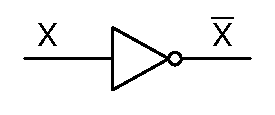
\includegraphics[scale=0.7]{logic/NOT.eps}
	\caption{The NOT gate, also called an inverter, outputs NOT(A).}
	\label{fig:notgate}
\end{figure} 

\begin{table}[!ht]
	\centering
	\begin{tabular}{| c | c |}
		\hline
		A & X \\ 
		\hline
		0 & 1 \\ \hline
		1 & 0 \\ \hline
	\end{tabular}
	\caption{This is the truth table for a NOT gate.}
	\label{table:notgate}
\end{table}

\begin{figure}[!htb]
	\centering
	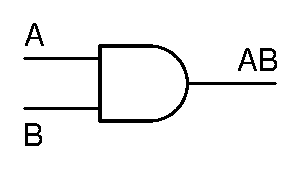
\includegraphics[scale=0.7]{logic/AND.eps}
	\caption{The AND gate outputs A AND B.}
	\label{fig:andgate}
\end{figure} 

\begin{table}[!ht]
	\centering
	\begin{tabular}{| c | c | c |}
		\hline
		A & B & X \\ 
		\hline
		0 & 0 & 0 \\ \hline
		0 & 1 & 0 \\ \hline
		1 & 0 & 0 \\ \hline
		1 & 1 & 1 \\ \hline
	\end{tabular}
	\caption{This is the truth table for an AND gate.}
	\label{table:andgate}
\end{table}

\begin{figure}[!htb]
	\centering
	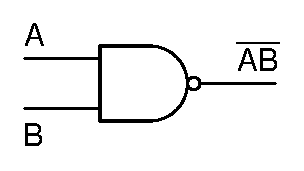
\includegraphics[scale=0.7]{logic/NAND.eps}
	\caption{The NAND gate outputs NOT(A AND B).}
	\label{fig:nandgate}
\end{figure} 

\begin{table}[!ht]
	\centering
	\begin{tabular}{| c | c | c |}
		\hline
		A & B & X \\ 
		\hline
		0 & 0 & 1 \\ \hline
		0 & 1 & 1 \\ \hline
		1 & 0 & 1 \\ \hline
		1 & 1 & 0 \\ \hline
	\end{tabular}
	\caption{This is the truth table for an NAND gate.}
	\label{table:nandgate}
\end{table}

\begin{figure}[!htb]
	\centering
	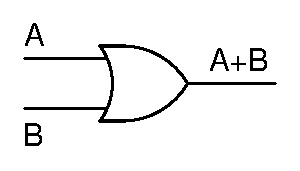
\includegraphics[scale=0.7]{logic/OR.eps}
	\caption{The OR gate outputs A OR B.}
	\label{fig:orgate}
\end{figure} 

\begin{table}[!ht]
	\centering
	\begin{tabular}{| c | c | c |}
		\hline
		A & B & X \\ 
		\hline
		0 & 0 & 0 \\ \hline
		0 & 1 & 1 \\ \hline
		1 & 0 & 1 \\ \hline
		1 & 1 & 1 \\ \hline
	\end{tabular}
	\caption{This is the truth table for an OR gate.}
	\label{table:orgate}
\end{table}

\begin{figure}[!htb]
	\centering
	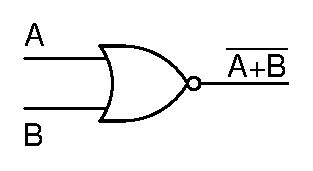
\includegraphics[scale=0.7]{logic/NOR.eps}
	\caption{The NOR gate outputs NOT(A OR B).}
	\label{fig:norgate}
\end{figure} 

\begin{table}[!ht]
	\centering
	\begin{tabular}{| c | c | c |}
		\hline
		A & B & X \\ 
		\hline
		0 & 0 & 1 \\ \hline
		0 & 1 & 0 \\ \hline
		1 & 0 & 0 \\ \hline
		1 & 1 & 0 \\ \hline
	\end{tabular}
	\caption{This is the truth table for an NOR gate.}
	\label{table:norgate}
\end{table}

	\chapter{Arduino Startup}
\chaplabel{arduino}

\section{Introduction}
This chapter gives the students an introduction to the hardware we are using and gets them started with 
the Arduino IDE.

\section{Datasheets}
\subsection{Arduino Nano Connect RP2040}
The data sheet for the Arduino Nano Connect RP2040 is located at\\ 
\href{https://docs.arduino.cc/resources/datasheets/ABX00053-datasheet.pdf}{https://docs.arduino.cc/resources/datasheets/ABX00053-datasheet.pdf}.

The main website for it is at \\
\href{https://docs.arduino.cc/hardware/nano-rp2040-connect}{https://docs.arduino.cc/hardware/nano-rp2040-connect}

The pinout is at \\
\href{https://content.arduino.cc/assets/Pinout\_NanoRP2040\_latest.png}{https://content.arduino.cc/assets/Pinout\_NanoRP2040\_latest.png}.

\subsubsection{RP2040 Microcontroller}
The RP2040 microcontroller datasheet (all 654 pages) is at \\
\href{https://datasheets.raspberrypi.com/rp2040/rp2040-datasheet.pdf}{https://datasheets.raspberrypi.com/rp2040/rp2040-datasheet.pdf}.

If you are ever interested in putting the microcontroller onto a circuit board yourself, there is a reference design at \\
\href{https://datasheets.raspberrypi.com/rp2040/hardware-design-with-rp2040.pdf}{https://datasheets.raspberrypi.com/rp2040/hardware-design-with-rp2040.pdf}.

\subsubsection{IMU - ST LSM6DSOXTR}
The IMU datasheet is at \\
\href{https://www.st.com/resource/en/datasheet/lsm6dsox.pdf}{https://www.st.com/resource/en/datasheet/lsm6dsox.pdf}

\subsubsection{Mic - ST MP34DT06JTR}
The microphone datasheet is at \\
\href{https://www.st.com/resource/en/datasheet/mp34dt06j.pdf}{https://www.st.com/resource/en/datasheet/mp34dt06j.pdf}

The \href{https://www.st.com/en/mems-and-sensors/mp34dt06j.html#sample-buy}{overview page} shows that the microphone is still actively being produced.

\subsubsection{WiFi and Bluetooth - U-blox® Nina W102}
The main page for the wireless unit is at \\
\href{https://www.u-blox.com/en/product/nina-w10-series-open-cpu}{https://www.u-blox.com/en/product/nina-w10-series-open-cpu}.

The datasheet is at \\
\href{https://www.u-blox.com/sites/default/files/NINA-W10\_DataSheet\_UBX-17065507.pdf}{https://www.u-blox.com/sites/default/files/NINA-W10\_DataSheet\_UBX-17065507.pdf}.

\subsubsection{Cryptographic IC - Microchip® ATECC608A}
Note that Microchip \href{https://www.microchip.com/en-us/product/ATECC608A}{doesn't suggest using this chip in new designs} so expect that some future versions of the
Nano RP2040 Connect to use the successor (\href{https://www.microchip.com/en-us/product/ATECC608B}{ATTECC608B}).

The datasheet for the 608A is here: \\
\href{https://ww1.microchip.com/downloads/en/DeviceDoc/ATECC608A-CryptoAuthentication-Device-Summary-Data-Sheet-DS40001977B.pdf}{https://ww1.microchip.com/downloads/en/DeviceDoc/ATECC608A-CryptoAuthentication-Device-Summary-Data-Sheet-DS40001977B.pdf}.

Note that it says it is a summary datasheet. You have to sign an NDA with Microchip to see the full datasheet.

\subsection{Circuit Board Parts (v0.5)}
\begin{enumerate}
    \item \href{https://datasheets.maximintegrated.com/en/ds/DS18B20.pdf}{DS18B20+ 1-Wire temperature sensor}
    \item \href{https://datasheet.lcsc.com/lcsc/2001041707_GXCAS-GX18B20_C472471.pdf}{GX18B20 1-Wire temperature sensor}
    \item \href{https://www.st.com/resource/en/datasheet/vl6180.pdf}{VL6180 Distance sensor}
    \item \href{https://sensirion.com/media/documents/213E6A3B/61641DC3/Sensirion_Humidity_Sensors_SHT3x_Datasheet_digital.pdf}{SHT31 Temperature and Humidity sensor}
    \item \href{https://ww1.microchip.com/downloads/en/DeviceDoc/21498D.pdf}{TC1047 Analog out temperature sensor}
    \item \href{https://www.ti.com/lit/ds/symlink/ads7142.pdf?ts=1660651868135}{ADS7142 Analog-to-digital converter (ADC)}
    \item \href{https://www.adafruit.com/product/4383}{Adafruit 1.14" 240x135 Color TFT Display + MicroSD Card Breakout - ST7789}
    \item \href{https://www.pololu.com/product/4012}{U3V40FX Voltage regulator}
    \item \href{https://datasheet.lcsc.com/lcsc/2001060933_TMI-TMI8837_C478955.pdf}{TMI8837 Motor controller}
    \item \href{https://datasheet.lcsc.com/lcsc/2012221837_QST-QMC5883L_C976032.pdf}{QMC5883L Compass}
    \item \href{https://www.st.com/resource/en/datasheet/st25dv16k.pdf}{ST25DV16 NFC I2C}
    \item \href{https://datasheet.lcsc.com/lcsc/2106062036_Worldsemi-WS2812B-B-W_C2761795.pdf}{NeoPixels (WS2812)}
    \item \href{https://www.nxp.com/docs/en/data-sheet/PCA9535_PCA9535C.pdf}{PCA9535 I2C GPIO}
    \item \href{https://datasheet.lcsc.com/lcsc/1810191633_SUNLIGHT-SLR0394FG3C5BD-3-5_C225905.pdf}{SLR0394 LED display}
\end{enumerate}

\section{Schematics and PCB}
\begin{landscape}
\begin{figure}[!htb]
	\centering
	%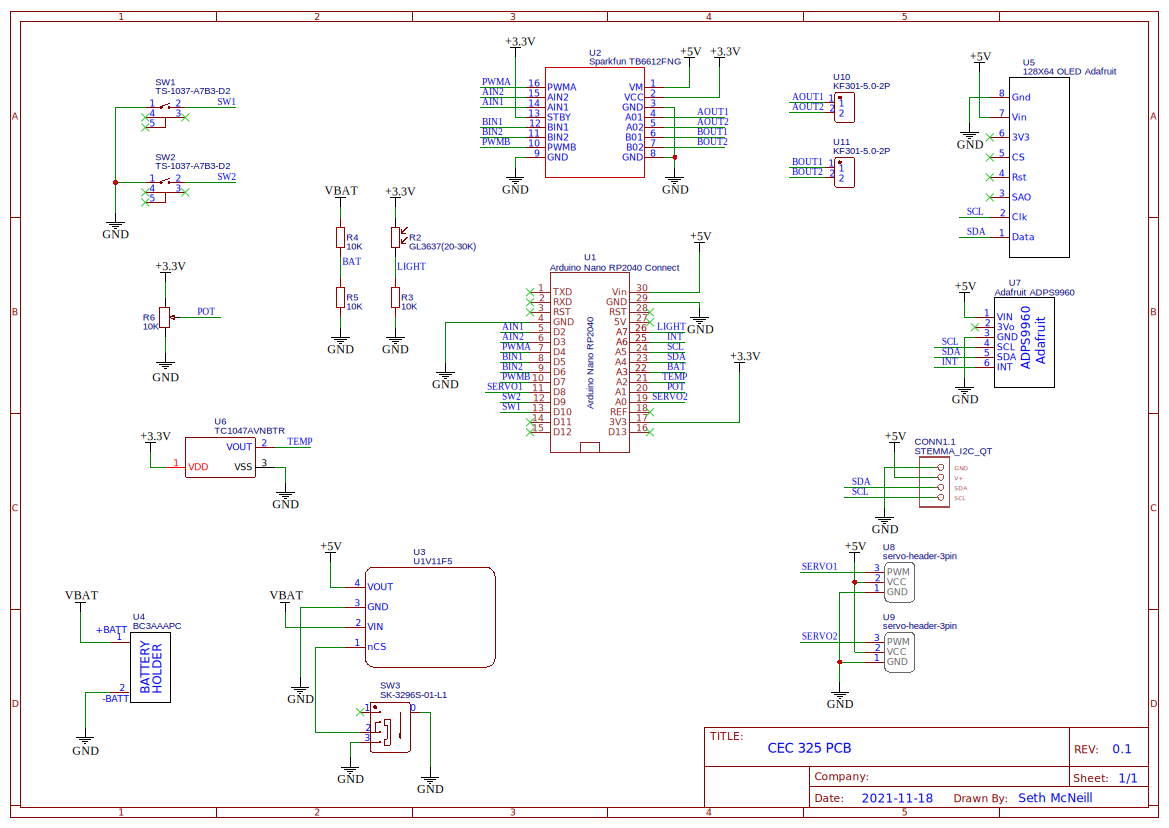
\includepdf[pages=-,pagecommand={},width=\textwidth]{arduinoStart/Schematic_NanoConnectRP2040test1_v0.1.pdf}
	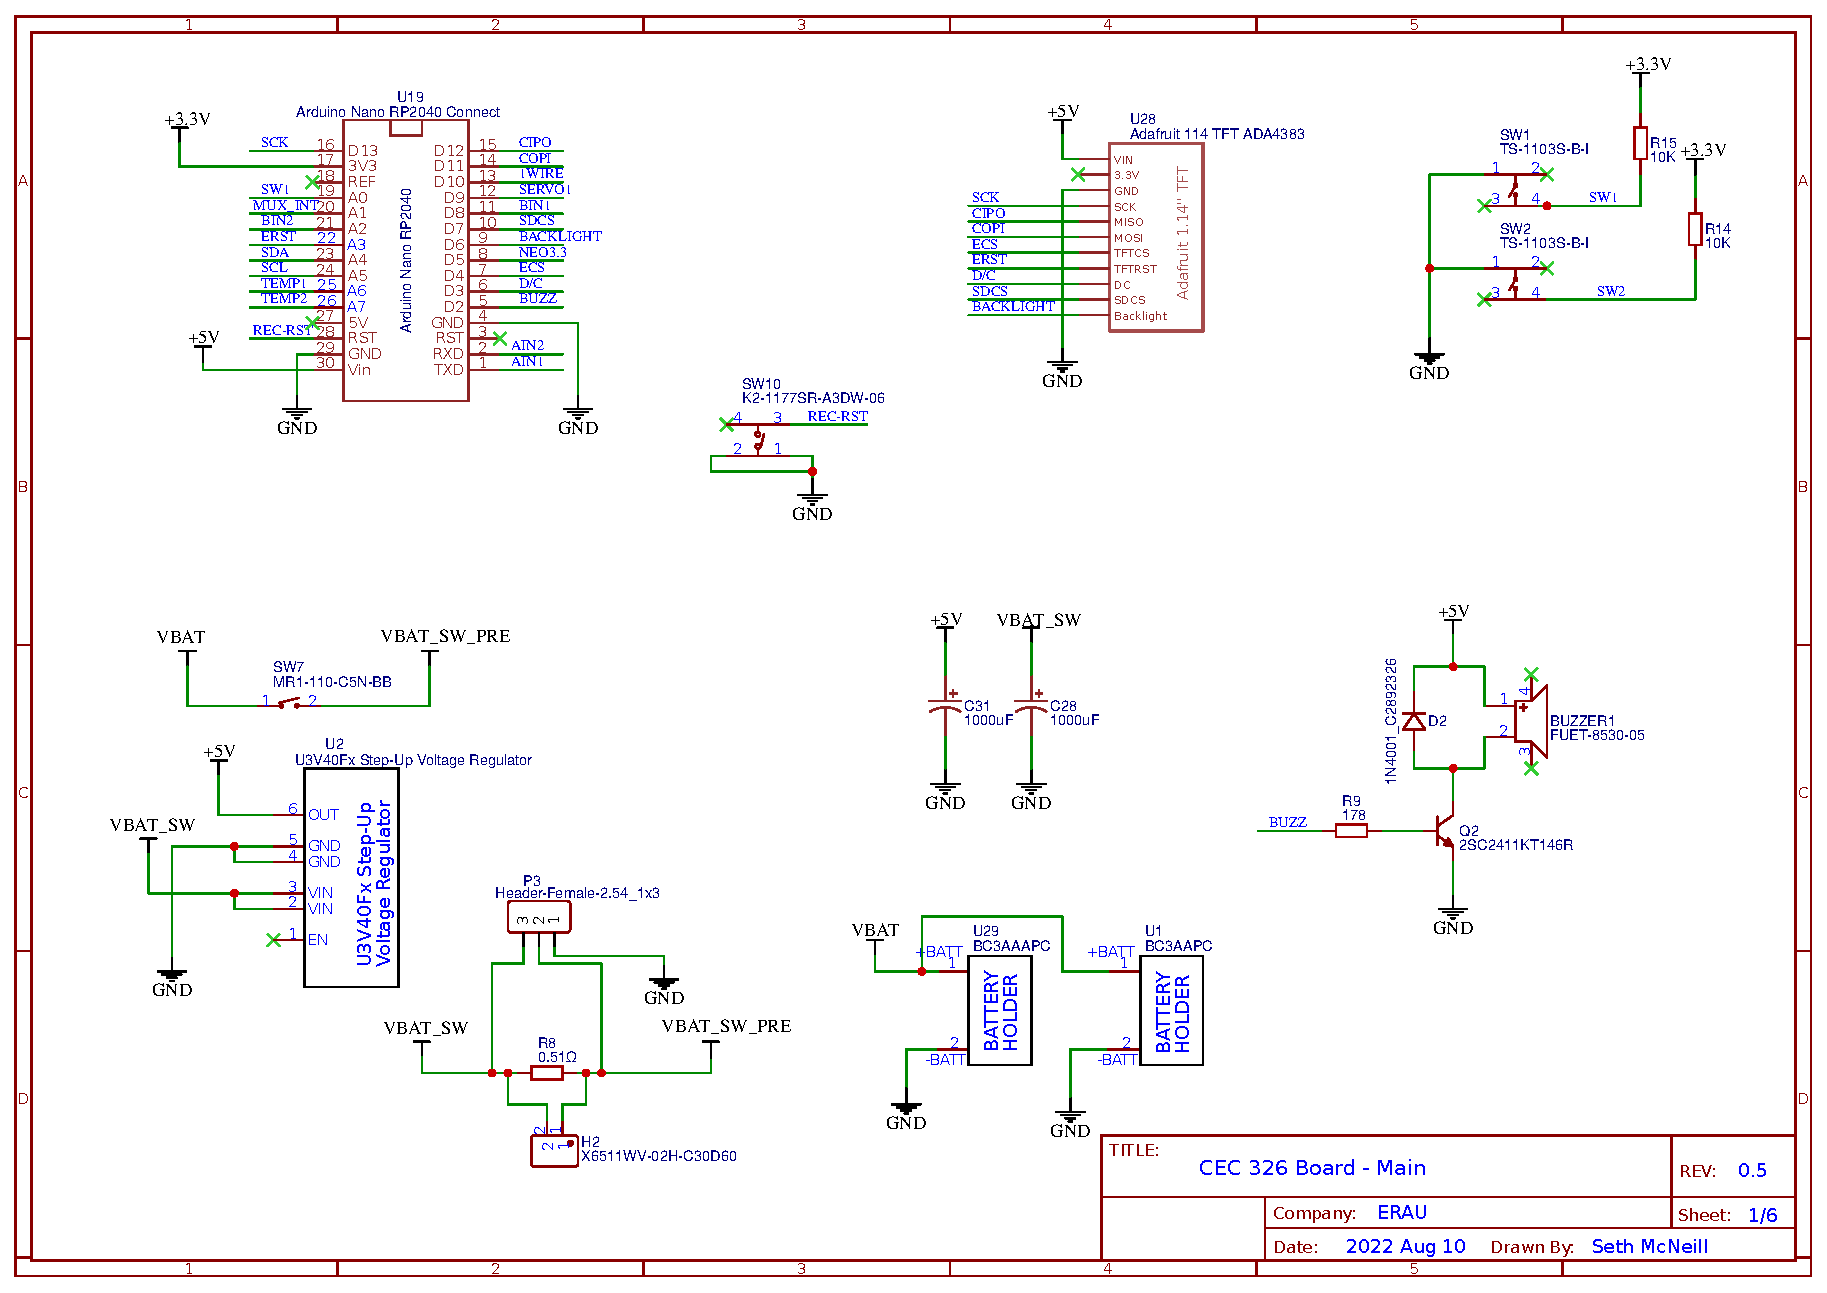
\includegraphics[width=\paperwidth]{arduinoStart/Schematic_CEC326v0.5_Main} % leaving off extension seems to work
	\caption{This is the schematic of version 0.3 of the board. This is the board used in Spring 2022.}
	\label{fig:boardSchematic}
\end{figure} 

\begin{figure}[!htb]
	\centering
	%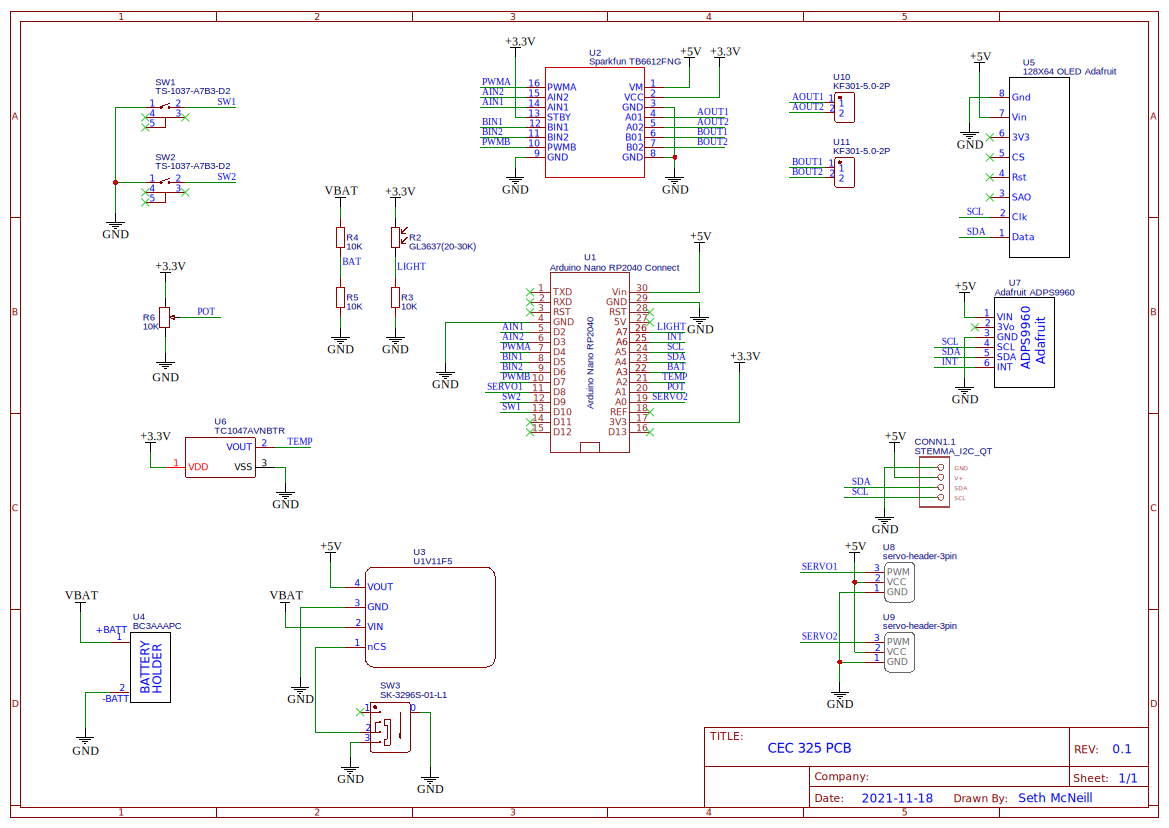
\includepdf[pages=-,pagecommand={},width=\textwidth]{arduinoStart/Schematic_NanoConnectRP2040test1_v0.1.pdf}
	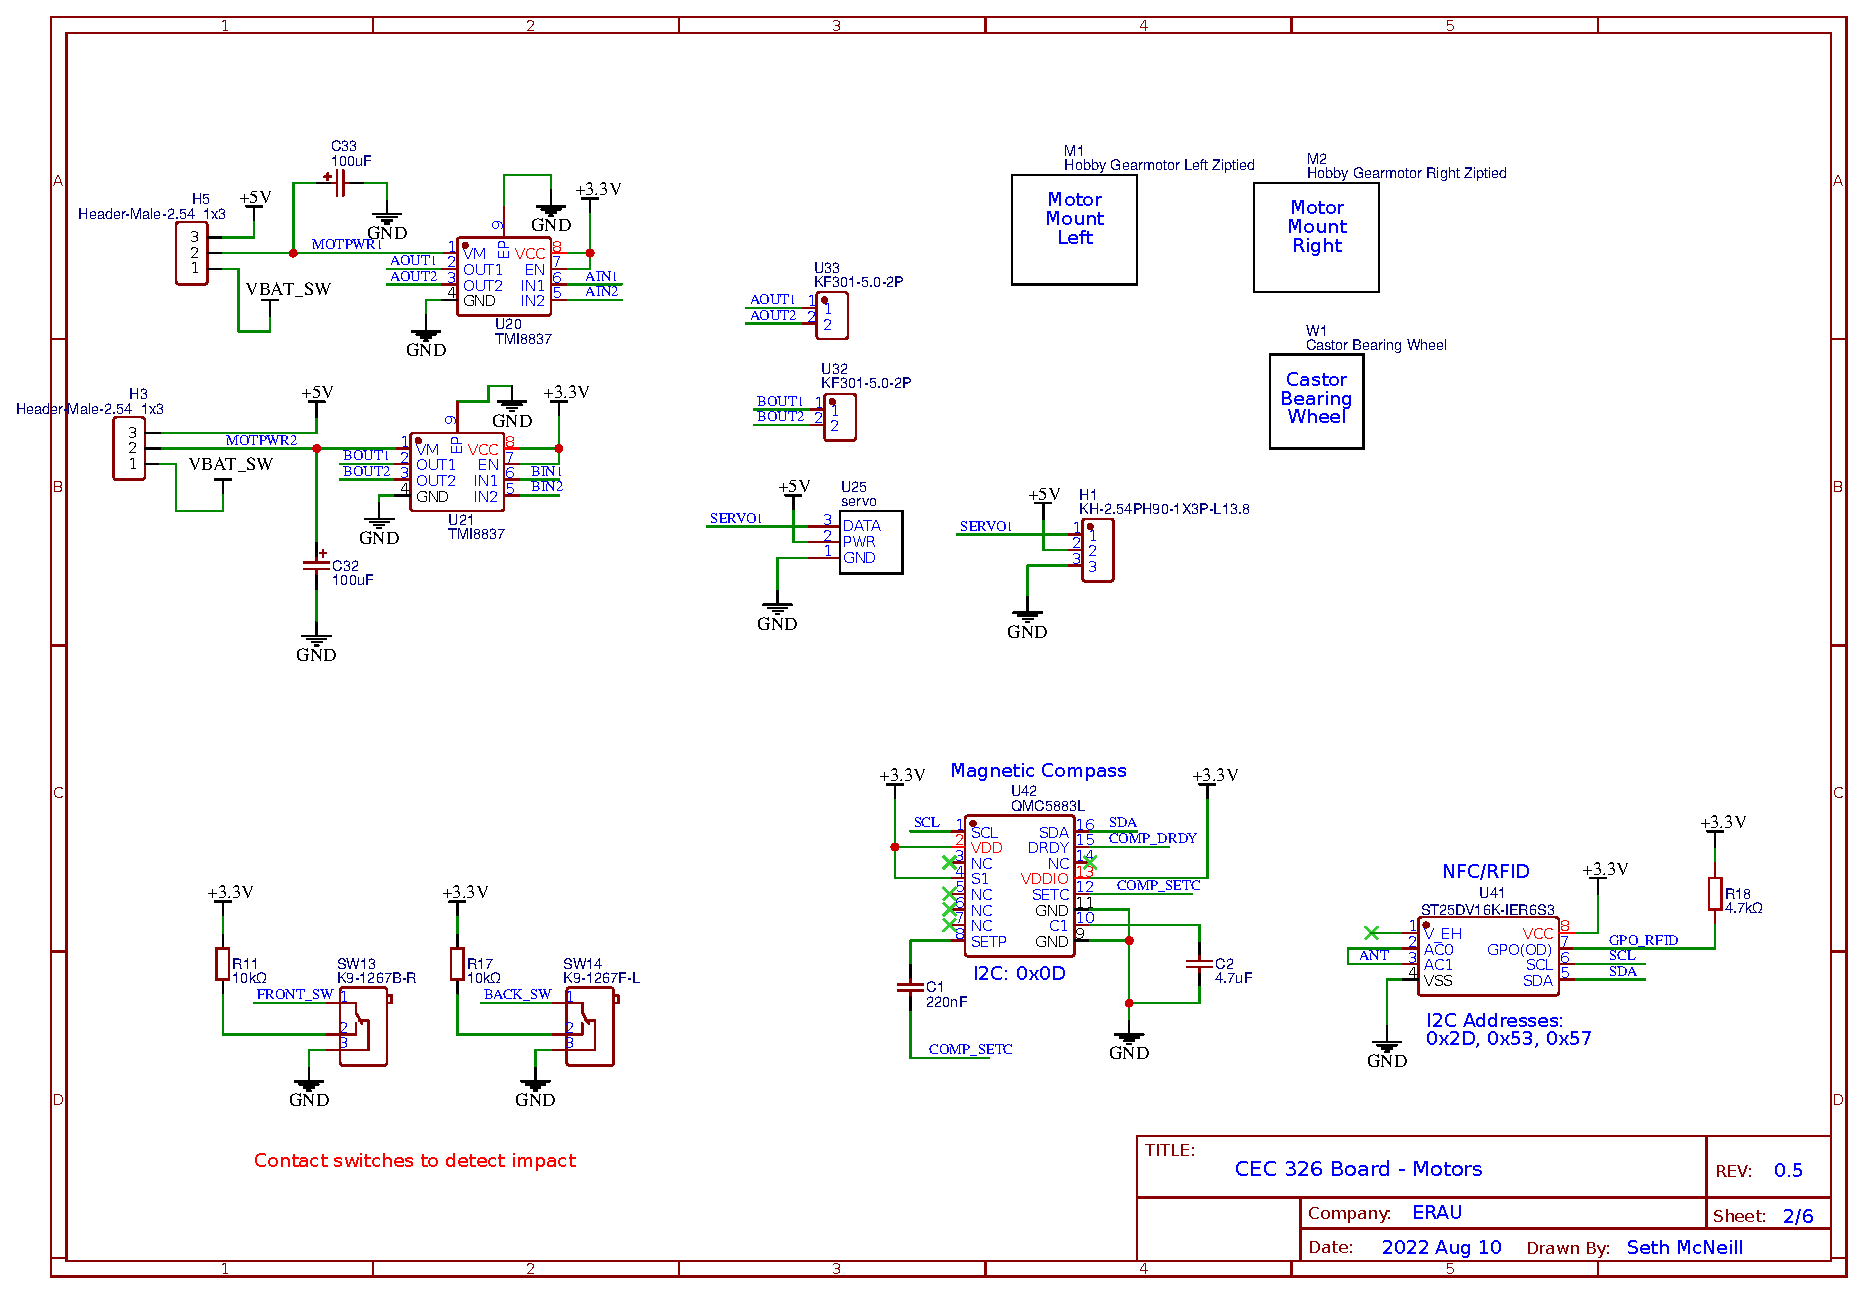
\includegraphics[width=\paperwidth]{arduinoStart/Schematic_CEC326v0.5_Motors} % leaving off extension seems to work
	\caption{This is the schematic of version 0.3 of the board. This is the board used in Spring 2022.}
	\label{fig:boardSchematic}
\end{figure} 

\begin{figure}[!htb]
	\centering
	%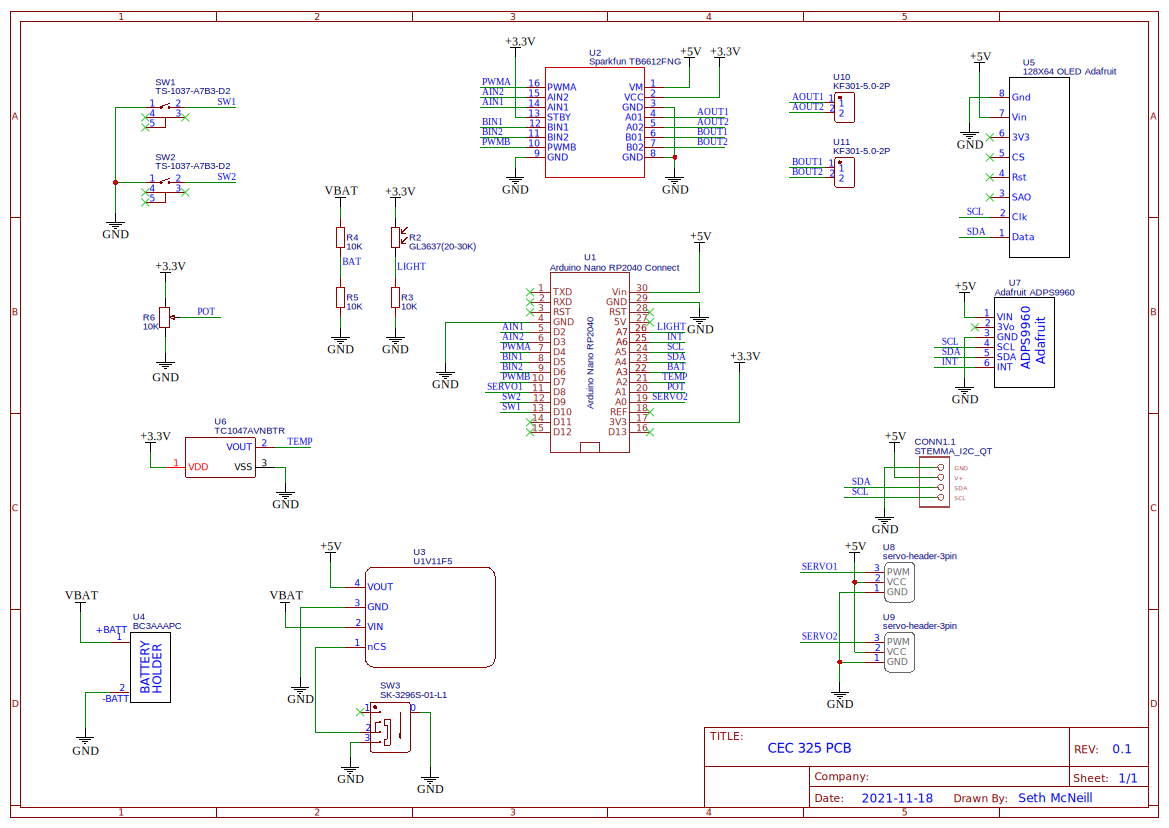
\includepdf[pages=-,pagecommand={},width=\textwidth]{arduinoStart/Schematic_NanoConnectRP2040test1_v0.1.pdf}
	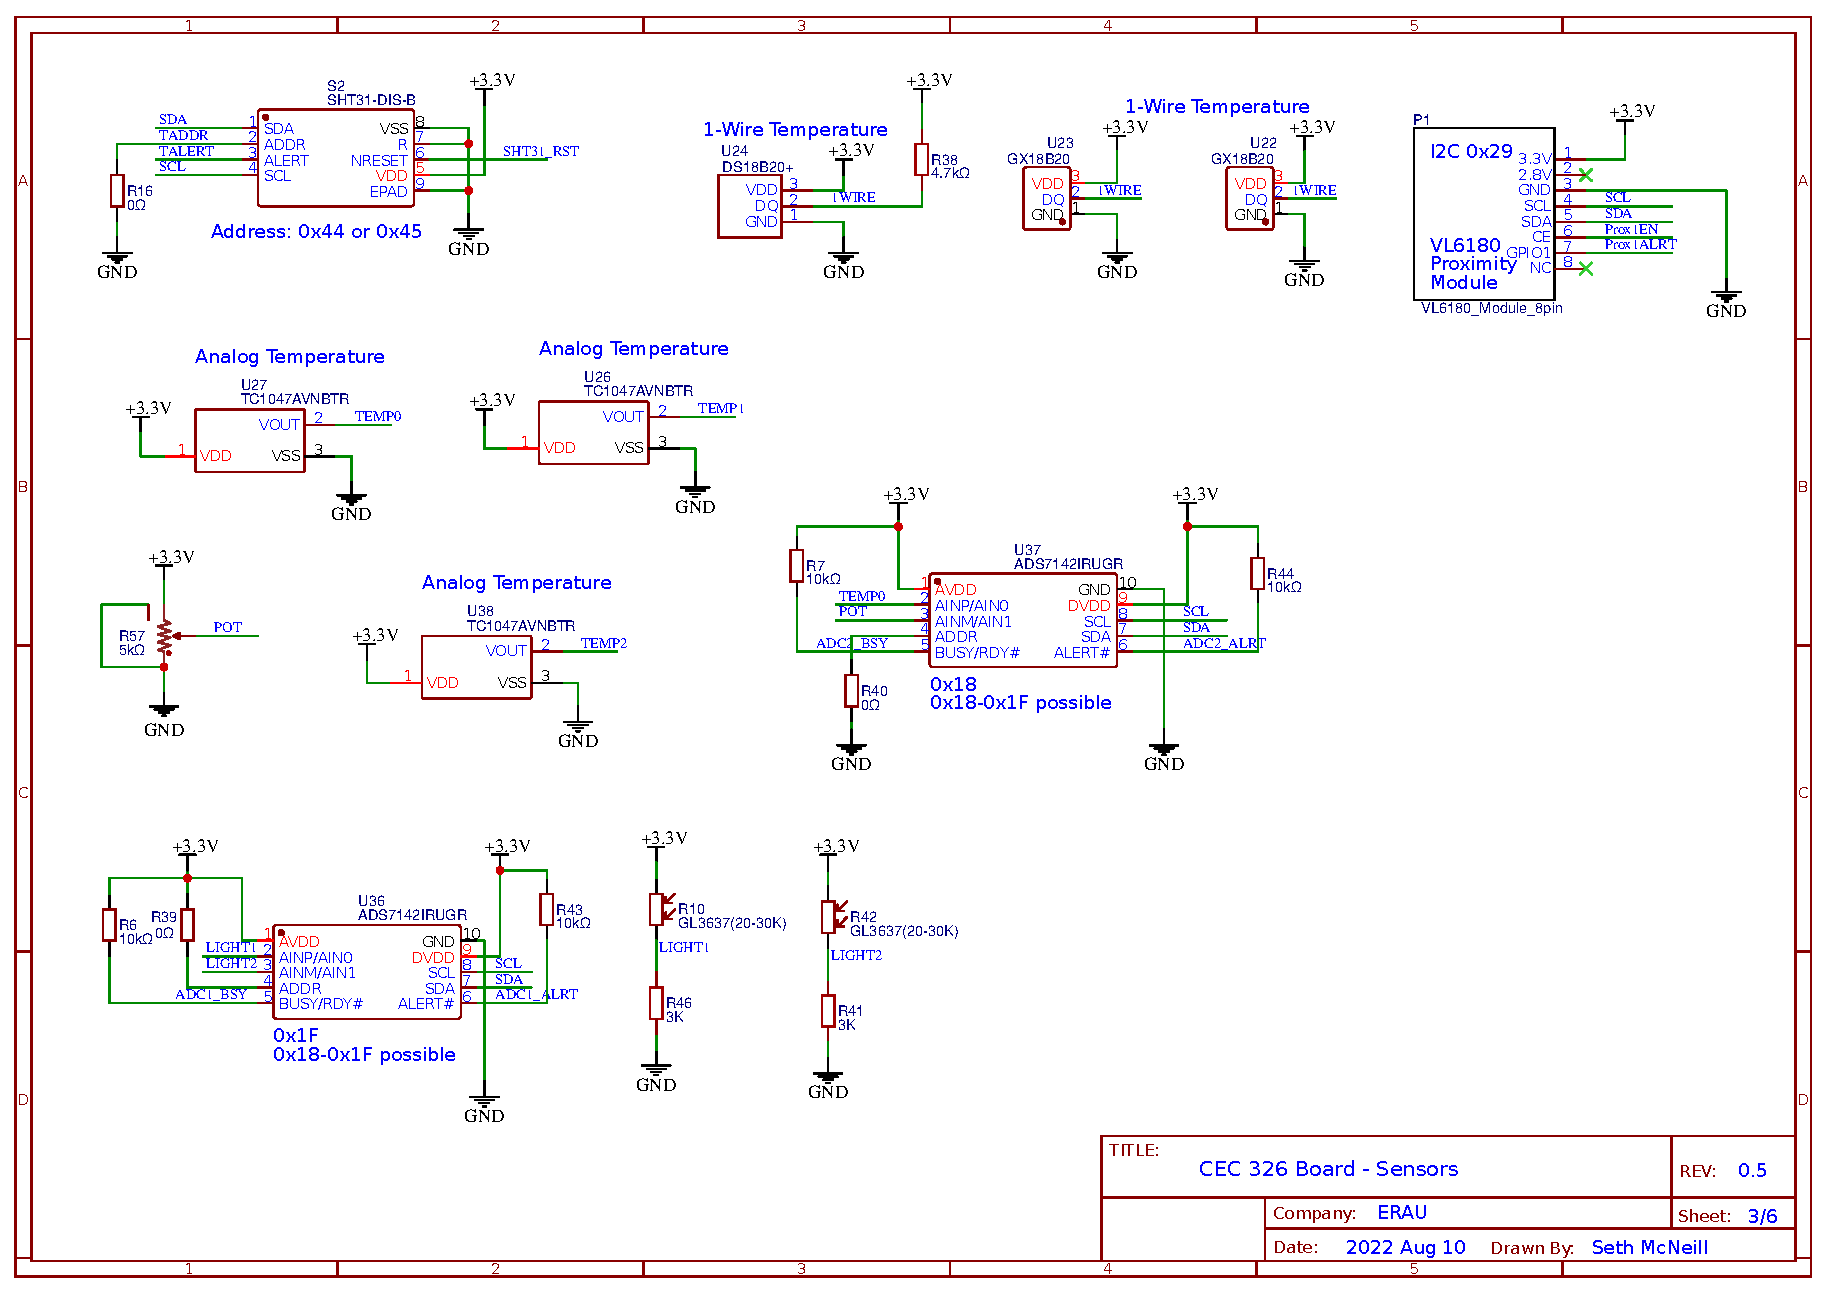
\includegraphics[width=\paperwidth]{arduinoStart/Schematic_CEC326v0.5_Sensors} % leaving off extension seems to work
	\caption{This is the schematic of version 0.3 of the board. This is the board used in Spring 2022.}
	\label{fig:boardSchematic}
\end{figure} 

\begin{figure}[!htb]
	\centering
	%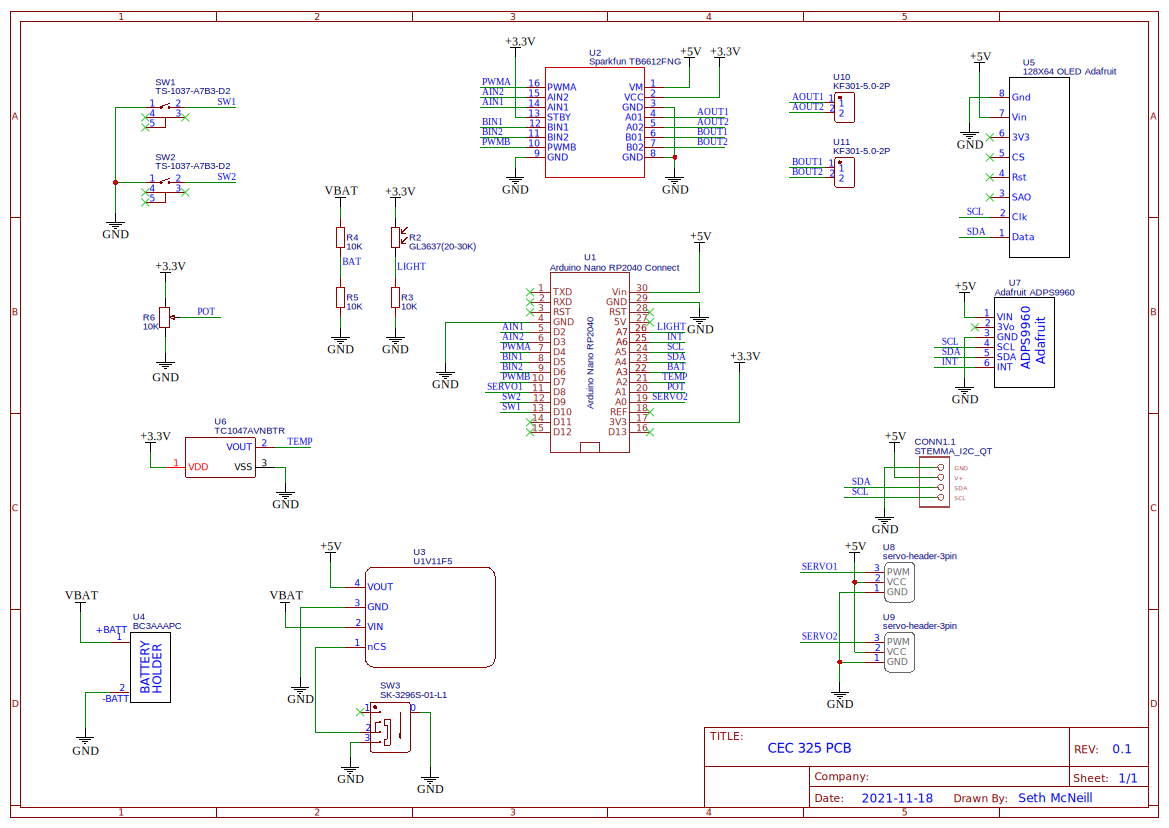
\includepdf[pages=-,pagecommand={},width=\textwidth]{arduinoStart/Schematic_NanoConnectRP2040test1_v0.1.pdf}
	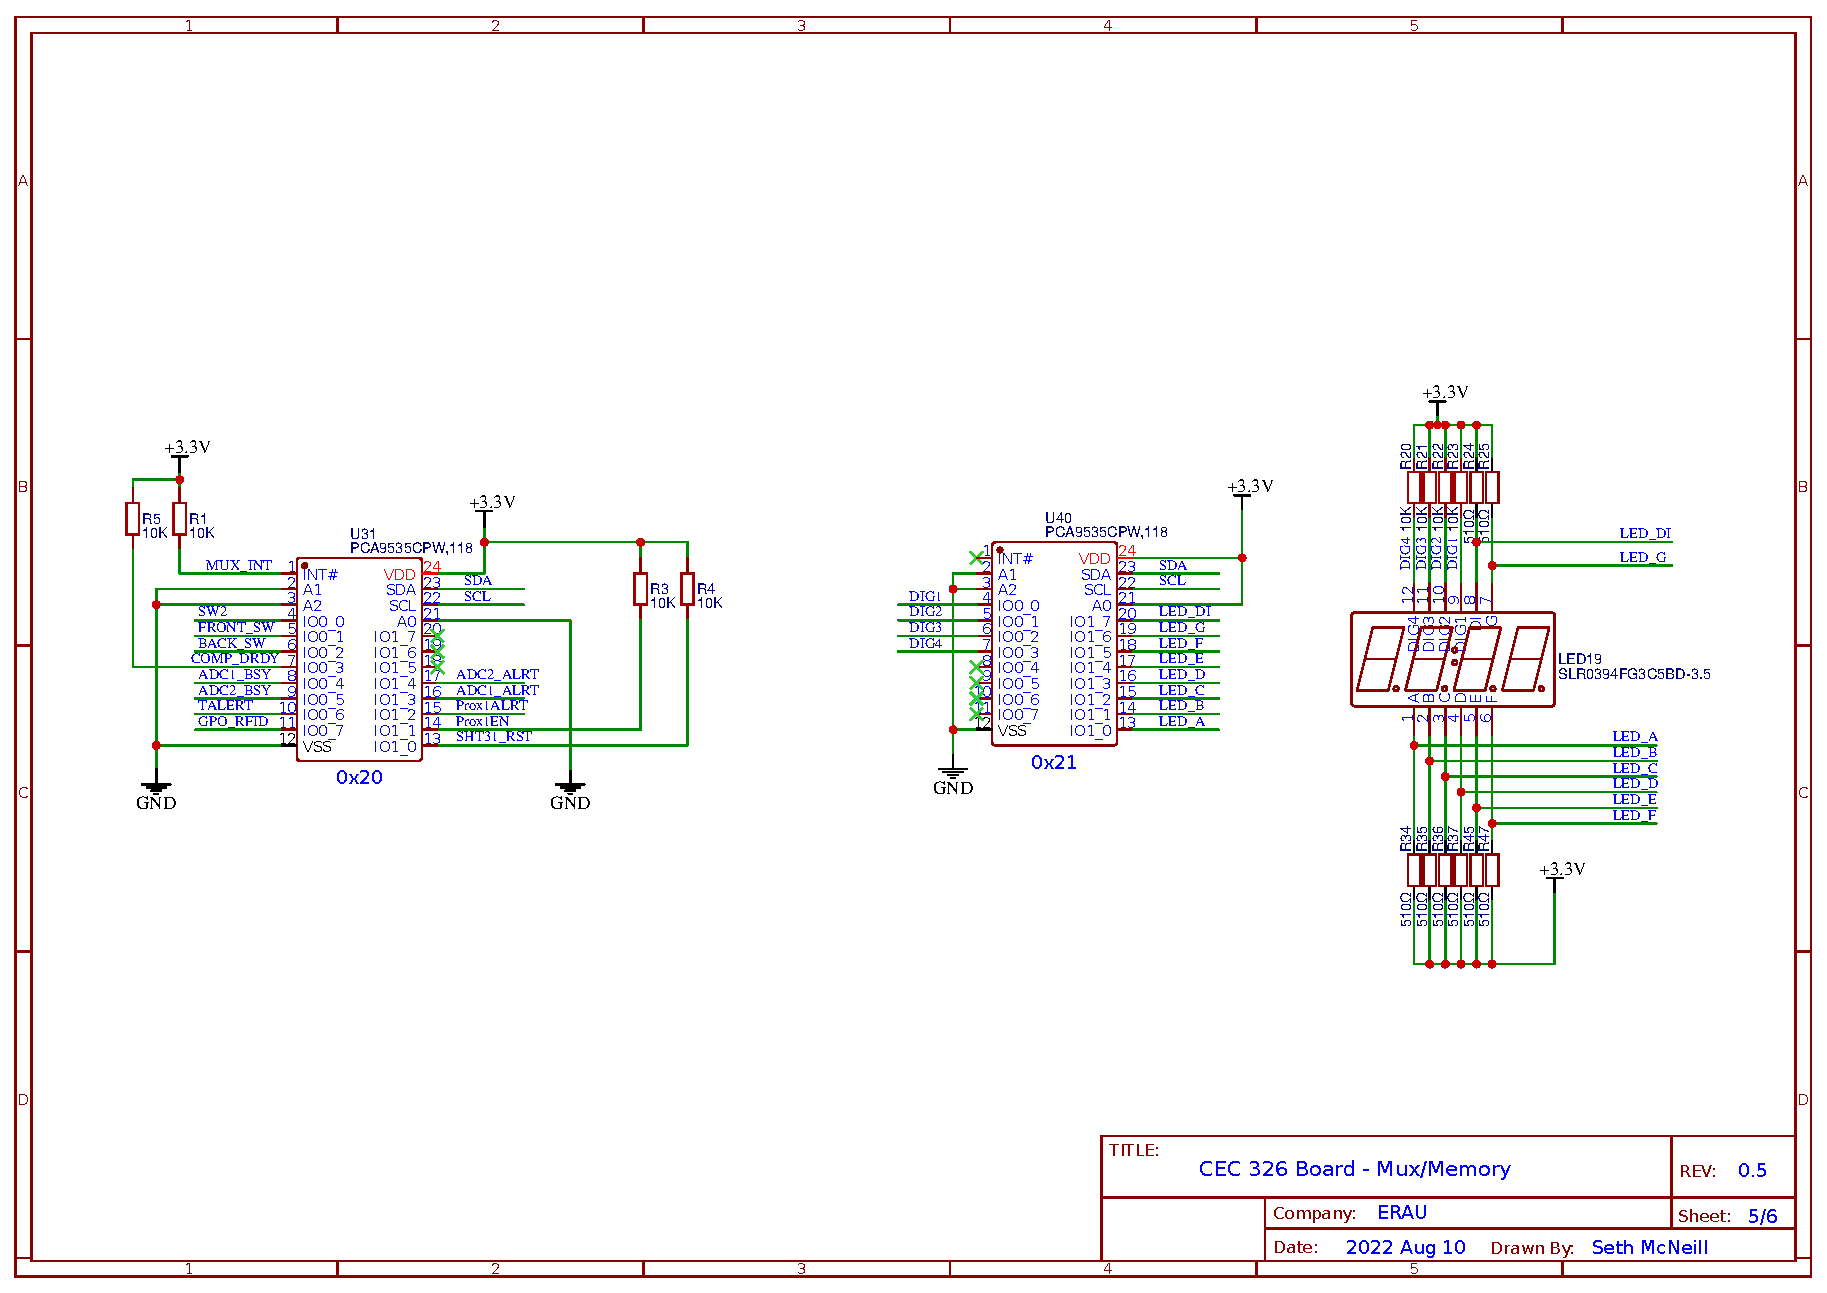
\includegraphics[width=\paperwidth]{arduinoStart/Schematic_CEC326v0.5_Mux} % leaving off extension seems to work
	\caption{This is the schematic of version 0.3 of the board. This is the board used in Spring 2022.}
	\label{fig:boardSchematic}
\end{figure} 

\begin{figure}[!htb]
	\centering
	%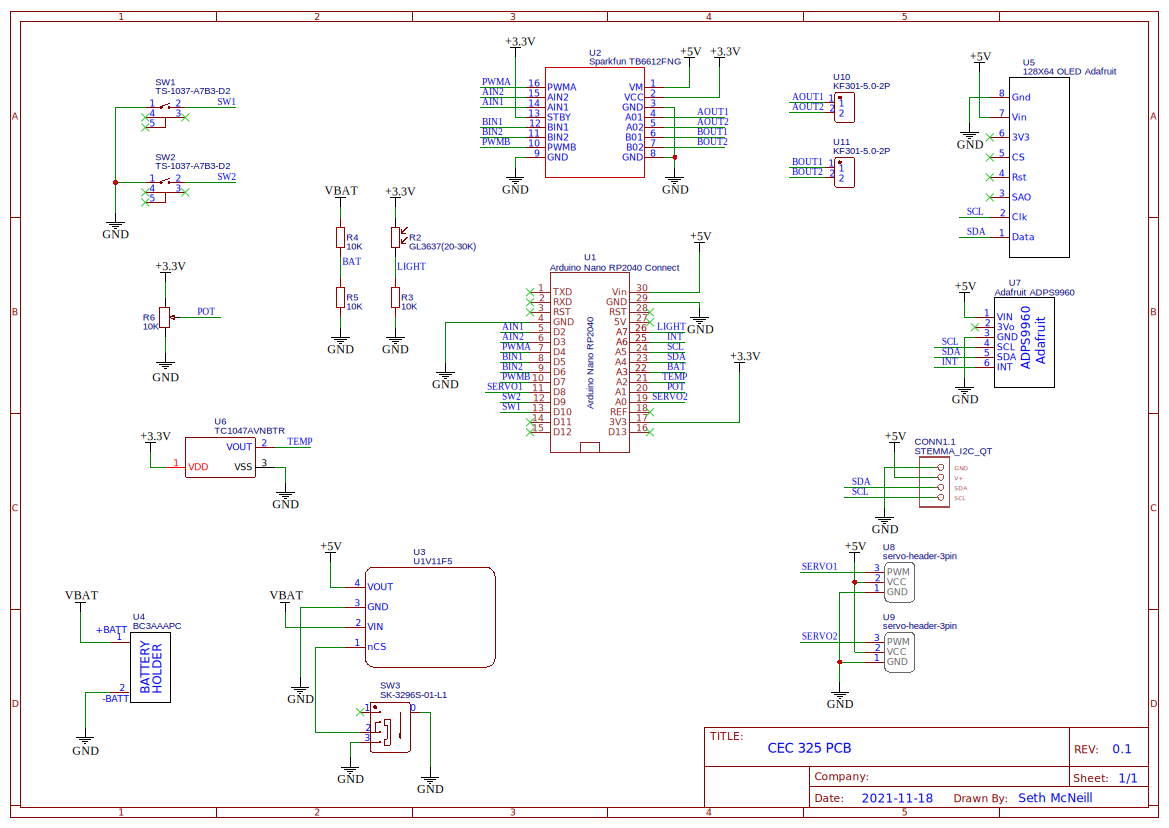
\includepdf[pages=-,pagecommand={},width=\textwidth]{arduinoStart/Schematic_NanoConnectRP2040test1_v0.1.pdf}
	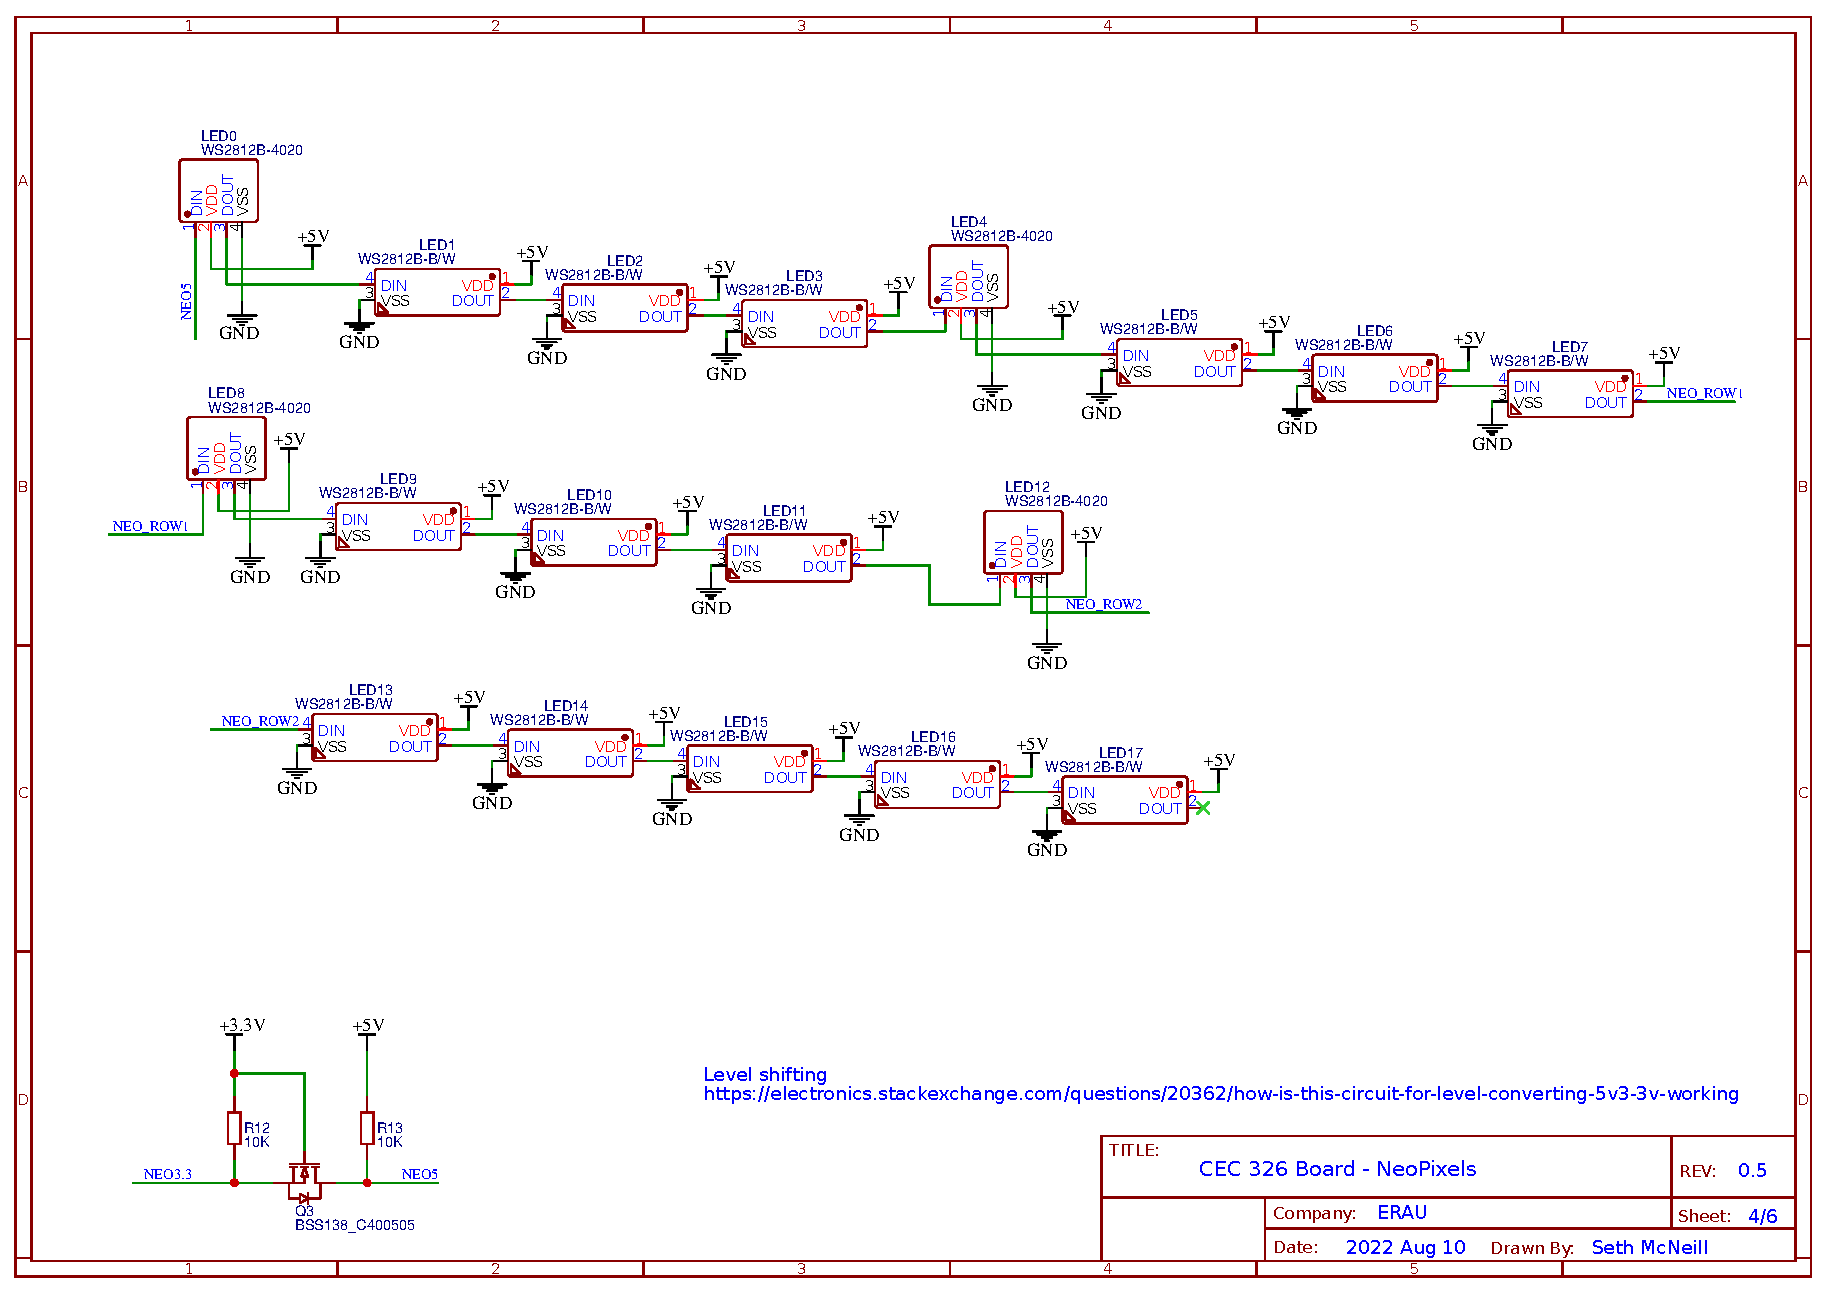
\includegraphics[width=\paperwidth]{arduinoStart/Schematic_CEC326v0.5_NeoPixels} % leaving off extension seems to work
	\caption{This is the schematic of version 0.3 of the board. This is the board used in Spring 2022.}
	\label{fig:boardSchematic}
\end{figure} 

\begin{figure}[!htb]
	\centering
	%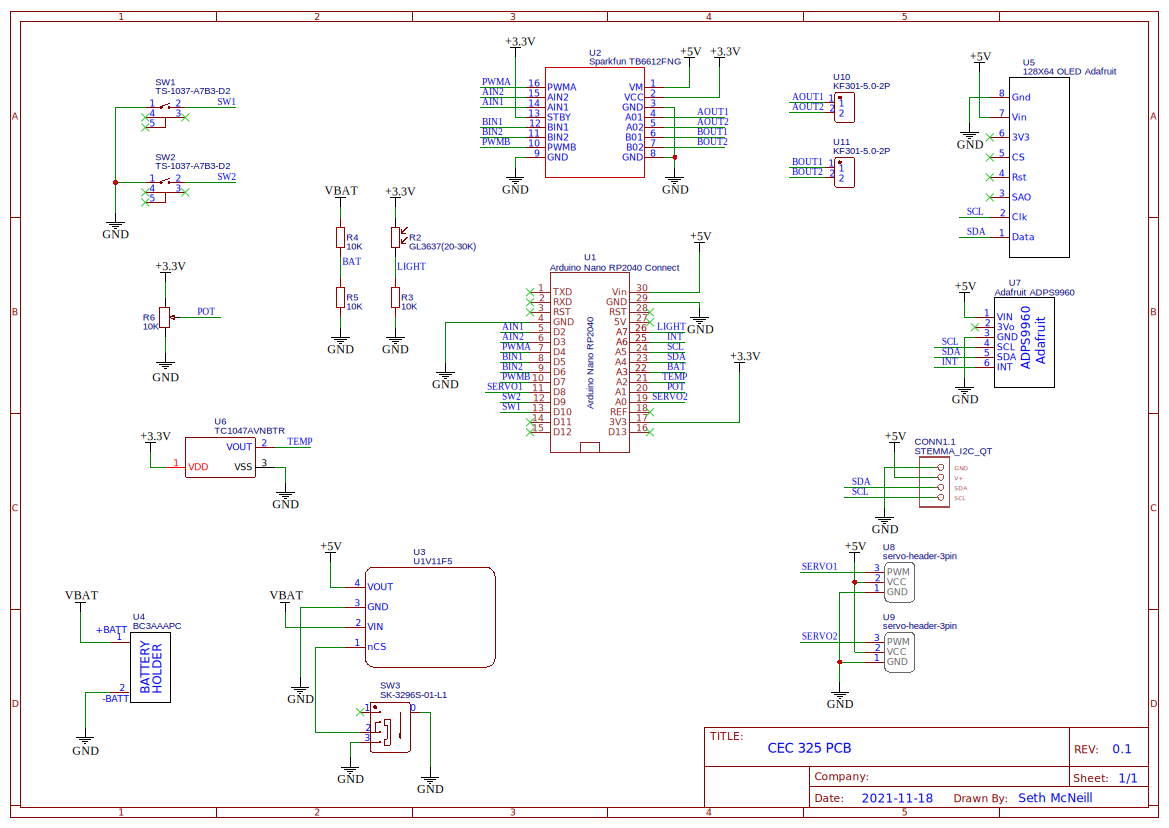
\includepdf[pages=-,pagecommand={},width=\textwidth]{arduinoStart/Schematic_NanoConnectRP2040test1_v0.1.pdf}
	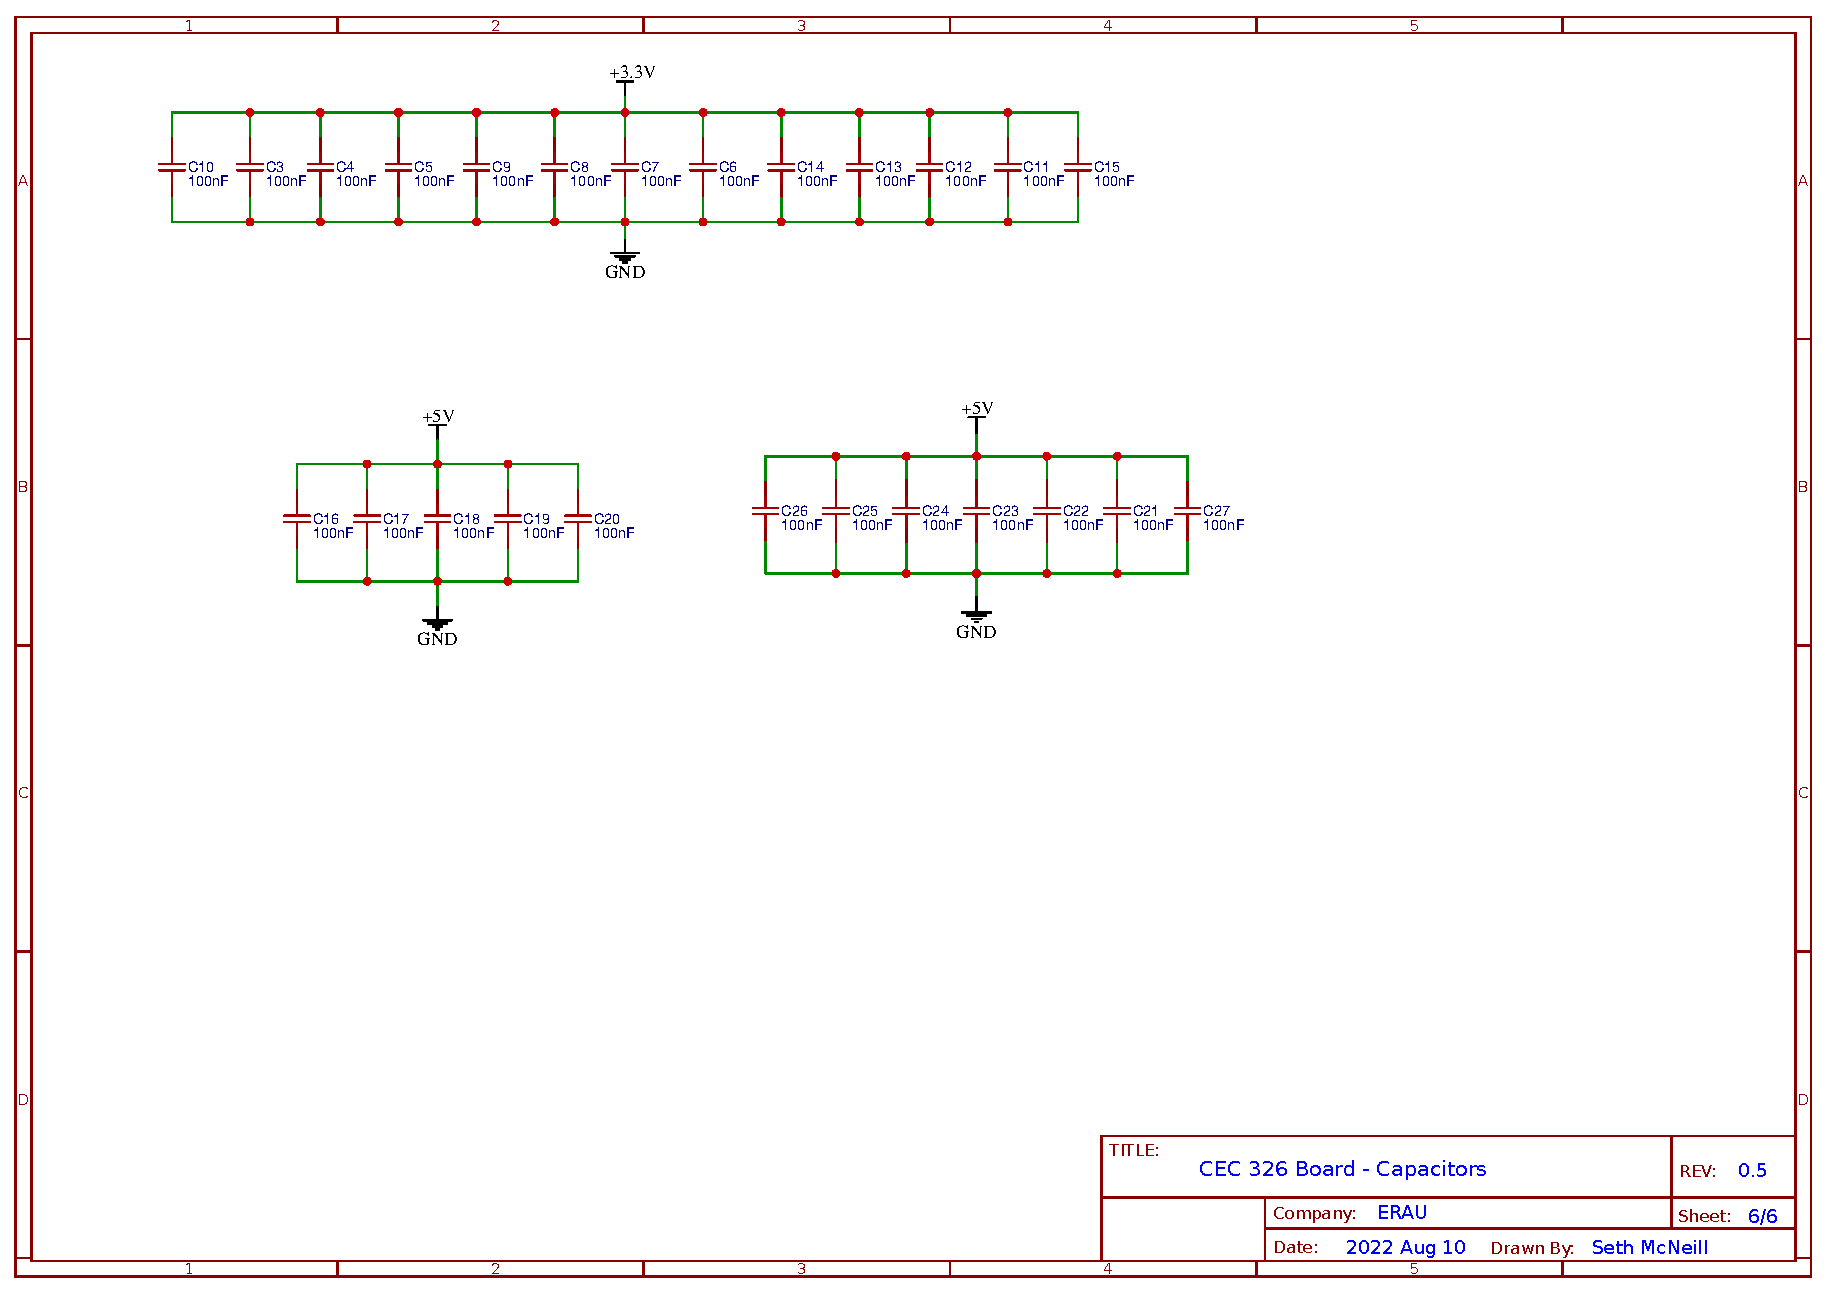
\includegraphics[width=\paperwidth]{arduinoStart/Schematic_CEC326v0.5_Caps} % leaving off extension seems to work
	\caption{This is the schematic of version 0.3 of the board. This is the board used in Spring 2022.}
	\label{fig:boardSchematic}
\end{figure} 

\end{landscape}

\begin{figure}[!htb]
	\centering
	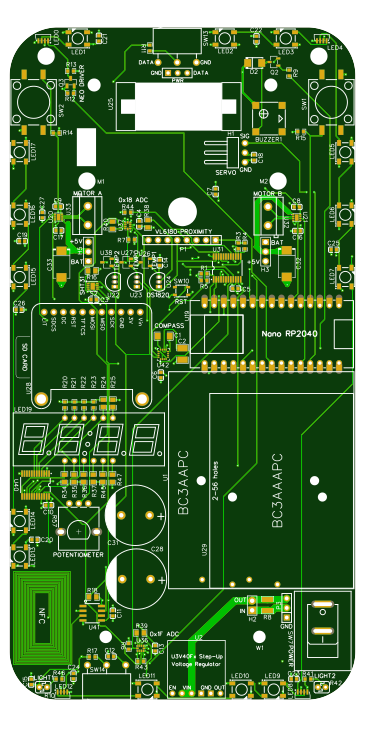
\includegraphics[scale=1.0]{arduinoStart/CEC326v0.5-PCB.png} % leaving off extension seems to work
	\caption{This shows the top of version 0.5 of the board for this class to help locate components.}
	\label{fig:boardTop}
\end{figure} 


	\chapter{Buttons and Serial Communications}
\chaplabel{buttons}

\section{Introduction}
This chapter introduces students to using buttons and serial communications.

\section{I2C}
I2C addresses for modules that are on the board or may be used with the board can be seen in Table \ref{table:i2caddresses}.

\begin{table}[!ht]
	\centering
	\begin{tabular}{l l}
		\hline
		Address (HEX) & Module \\ 
		\hline
		0x44 or 0x45 & SHT31-DIS Temperature/Humidity \\
		0x3D & 1.3" 128x64 OLED Display \\
		0x39 & APDS-9960 Light, Color, Proximity, Gesture \\
		0x77 & BME688 Temperature, Humidity, Gas \\
		0x2D, 0x53, and 0x57 & ST25DV16 Dynamic NFC/RFID Tag IC \\
		0x30 or other  & NeoKey 1x4 QT breakout board \\
		0x10 & STEMMA MiniGPS \\
		\hline
	\end{tabular}
	\caption{I2C addresses for relevant modules.}
	\label{table:i2caddresses}
\end{table}
	\chapter{Displays}
\chaplabel{displays}

\section{Introduction}
Adding a display to a device allows much more information to be shared from the device to the user than 
just using LEDs or buzzers. There are several types of displays that are commonly used in the embedded systems 
world. 

\subsection{LCD}
The most common is a Liquid Crystal Display (LCD). Most of the computer monitors and computers are LCD. This 
technology gives good contrast, fast response (which gamers like), and minimal burn in. Old CRT displays had 
to have screensavers so that whatever was usually showing on the display wouldn't be there permanently. 
Thankfully modern displays don't typically have this problem. LCDs do require a backlight. This determines
how bright the colors are. The pixels in the display just modulate how much of the backlight is showing.

At times you will find TFT displays. This stands for thin-film-transistor liquid-crystal display. They are 
a better version of LCD.

\subsection{eInk}
eInk displays are also available for embedded systems. These displays are of particular interest because they keep their 
display even when the power is turned off. This allows for very low power operations. The downsides are 
that they work off of reflected light so require special backlighting to be viewed at night and that 
they are very slow. A small display may take several seconds to refresh and some recommend not to update
them more than once every few minutes if possible.

\subsection{OLED}
The cool part about Organic Light Emitting Diode (OLED) displays is that  
instead of each pixel blocking the backlight to make the display like in LCDs, in 
OLED displays each pixel is an LED that emits light. This makes OLED displays very bright with very 
good contrast ratios. They also have fast response times. Some OLED displays will get dimmer with time. 
\href{https://www.adafruit.com/product/938}{Adafruit notes} that for their small 
OLED displays the dimming becomes noticeable after about 1000~hours of being on. This is 41.7~days, 
so after a year of continuous use, an OLED display might not be very bright.

\section{Pixel Layout}
The layout of pixels on a display can be thought of as a cartesian coordinate system with a couple 
minor differences. First, pixels take up space, so the indexing is between the lines rather than 
on the lines. Second, the +Y axis points downward as shown in Figure \ref{fig:pixels}. The units
for the coordinates is always pixels and the coordinates are always integers. 

Pixels can vary in size. This is important to keep in mind if you are trying to display something
with a specific size. Pixel size varies from display to display so read carefully if you want 
something to display a specific size.

\newcommand*{\xMin}{0}%
\newcommand*{\xMax}{6}%
\newcommand*{\yMin}{0}%
\newcommand*{\yMax}{6}%
\begin{figure}[!htb]
	\centering
	\begin{tikzpicture}

		\node[anchor=west] at (0,6.75) {\large$x\rightarrow$};
		\node[anchor=west,rotate=-90] at (-0.75,6) {\large$y\rightarrow$};

		\foreach \i in {\xMin,...,\xMax} {
			\draw [very thin,gray] (\i,\yMin) -- (\i,\yMax);
		}
		%https://tex.stackexchange.com/questions/36713/computing-in-the-list-of-a-tikz-foreach
		\foreach \i in {\xMin,...,\number\numexpr\xMax-1\relax} {
			\node[anchor=south] at (\i+0.5,\yMax) {$\i$}; 
		}
		\foreach \i in {\yMin,...,\yMax} {
			\draw [very thin,gray] (\xMin,\i) -- (\xMax,\i);
		}
		\foreach \i in {\yMin,...,\number\numexpr\yMax-1\relax} {
			\node[anchor=east] at (\xMin,\yMax - \i-0.5) {$\i$}; 
		}
		\fill [gray] (3,3) rectangle (4,4);
		\node[anchor=center] at (3.5,3.5) {\color{white}(3,2)};
		\fill [gray] (1,1) rectangle (2,2);
		\node[anchor=center] at (1.5,1.5) {\color{white}(1,4)};
	\end{tikzpicture}
	\caption{Pixels in a display occupy space are are referenced to the top left corner with the positive Y axis going down.}
	\label{fig:pixels}
\end{figure}

\section{Using the Display}
The display on the lab board is a 1.14" TFT display 240~pixels wide and 135~pixels high. 
Two libraries are required to use it:
\begin{enumerate}
	\item \lstinline@Adafruit_GFX.h@ - this is the generic graphics library
	\item \lstinline@Adafruit_ST7789.h@ - this is specific to our display
\end{enumerate}
An example that shows much of the available functionality can be found (once the libraries are installed)
at Examples $\rightarrow$ Adafruit ST7735 and ST7789 Library $\rightarrow$ graphicstest\_st7789. 
The following have to be defined to use a display:
\begin{enumerate}
	\item Width - how many pixels wide the display is 
	\item Height - how many pixels high the display is 
	\item Reset pin - Allows the microcontroller to reset the display
	\item CS - Chip Select, used by SPI to select the display when communicating
	\item DC - Data/Command pin used to determine the type of data being sent to the display
\end{enumerate}

An example of creating a display instance is as follows:\\
\lstinline@Adafruit_ST7789 tft = Adafruit_ST7789(TFT_CS, TFT_DC, TFT_RST);@

Some useful methods that can be called on the display object are:
\begin{enumerate}
	\item fillScreen - Fills the screen with the specified color. Usually used to clear the screen.
	\item setTextSize - sets the size of the text (usually 2-4)
	\item setTextColor - set what color the text should be. Some examples are 
	\begin{enumerate}
        \item ST77XX\_BLACK
        \item ST77XX\_BLUE
        \item ST77XX\_RED
        \item ST77XX\_YELLOW
    \end{enumerate}
	\item print/println - these act the same as they do when using Serial
	\item drawBitmap - draws a bitmap stored using PROGMEM or a canvas. It requires the following arugments
	\begin{enumerate}
		\item xpos - the x position for the image
		\item ypos - the y position for the image
		\item bitmap variable - the variables with the actual image
		\item width - image width in pixels
		\item height - image height in pixels 
	\end{enumerate}
	\item More can be \href{https://learn.adafruit.com/adafruit-gfx-graphics-library/graphics-primitives}{found here}.
\end{enumerate}

\subsection{Using Canvas to Reduce Flicker}
Redrawing by calling \lstinline@fillScreen()@ causes a flicker that can be 
problematic. The solution is to create a canvas in memory that the program
draws to and then copy it over to the display using \lstinline@drawBitmap@. 
This technique does require that the microcontroller have enough memory to 
store the canvas.

The method requires creating a canvas variable, drawing everything to the canvas
and then copying the canvas over to the display. Listing \ref{lst:canvasdisplay}
shows the basics of this method.


\begin{lstlisting}[language=C++, caption={Snippets showing how to use a canvas to 
    reduce flicker when updating a display.},label={lst:canvasdisplay}]
    // unlike the online example, 
    //this is a 16-bit color canvas
    GFXcanvas16 canvas(240,135);
    ...
    canvas.fillScreen(ST77XX_BLACK);  // clear canvas
    canvas.setCursor(0,0);
    canvas.setTextSize(3);
    canvas.println("Hello world!");
    tft.drawRGBBitmap(0, 0, canvas.getBuffer(),
        240, 135);  // copy canvas to display
\end{lstlisting}
	\chapter{Sampling and Data Collection}
\chaplabel{data}

\section{Introduction}
This chapter introduces students to the concepts of Analog-to-Digital Converters (ADCs) and data collection.

\section{Sampling}

The real world has signals that are continuous in both time and amplitude. Unfortunately, microcontrollers 
do not have continuous time or amplitude capabilities. This means that real signals have to be quantized 
in amplitude and sampled in time before they can be analyzed by a microcontroller. Figure \ref{fig:quantized}
shows what quantization in amplitude looks like. The microcontroller can only see values of -3 to +3 in 
this example even though the real signal has values between these. Figure \ref{fig:quantizederror} 
includes the errors incurred due to quantization.

\begin{figure}[!htb]
	\centering
	\includegraphics[scale=0.5]{dataCollection/quantized.eps}
	\caption{This shows amplitude quantization.}
	\label{fig:quantized}
\end{figure}

\begin{figure}[!htb]
	\centering
	\includegraphics[scale=0.5]{dataCollection/quantizedError.eps}
	\caption{This shows amplitude quantization and the resulting error.}
	\label{fig:quantizederror}
\end{figure}

Sampling in the time domain could be done in a random fashion as demonstrated in Figure \ref{fig:randsample}
but that is rarely a good idea. The math that can be done with a signal that is sampled at an even rate 
as shown in Figure \ref{fig:evensampling} is very powerful. Therefore, we try very hard to sample at 
a specific frequency with minimal jitter in the time between samples.

\begin{figure}[!htb]
	\centering
	\includegraphics[scale=0.5]{dataCollection/randomSampling.eps}
	\caption{This shows random sampling.}
	\label{fig:randsample}
\end{figure}

\begin{figure}[!htb]
	\centering
	\includegraphics[scale=0.5]{dataCollection/evenSampling.eps}
	\caption{This shows even sampling.}
	\label{fig:evensampling}
\end{figure}

A signal that has been both quantized and sampled is shown in Figure \ref{fig:samplequantized}. The 
signal has been reduced to the sequence of numbers: \{0,3,3,0,-3,-2\}.

\begin{figure}[!htb]
	\centering
	\includegraphics[scale=0.5]{dataCollection/sampledAndQuantized.eps}
	\caption{This shows a sampled and quantized signal.}
	\label{fig:samplequantized}
\end{figure}

It is important to sample fast enough to actually capture the signal of interest. The minimum 
sampling rate to capture a particular signal is called the  
\href{https://en.wikipedia.org/wiki/Nyquist_frequency}{Nyquist rate or Nyquist frequency}. The 
sampling rate for a signal must be at least twice the highest frequency in the signal in order 
to correctly see the signal in a sampled system. Figure \ref{fig:nyquist1} shows the best case 
when sampling at exactly twice the frequency of the signal. This can be noted since there are 
two sample points in one period of the sine wave. The worst case of sampling at exactly the 
Nyquist rate is shown in Figure \ref{fig:nyquist2}. A zoomed out version is shown in 
Figure~\ref{fig:nyquist3}. This is why it is best to give a little overhead when choosing 
the sample rate to use on a signal. If that is done, it yields Figure~\ref{fig:nyquist4} where 
the sampling rate is just a little over the frequency of the sine wave.

\begin{figure}[!htb]
	\centering
	\includegraphics[scale=0.5]{dataCollection/nyquist1.eps}
	\caption{This is the best case when sampling at the Nyquist rate.}
	\label{fig:nyquist1}
\end{figure}

\begin{figure}[!htb]
	\centering
	\includegraphics[scale=0.5]{dataCollection/nyquist2.eps}
	\caption{This is the worst case when sampling at exactly the Nyquist rate.}
	\label{fig:nyquist2}
\end{figure}

\begin{figure}[!htb]
	\centering
	\includegraphics[scale=0.5]{dataCollection/nyquist3.eps}
	\caption{This is a zoomed out view of the worst case of sampling at exactly the Nyquist rate.}
	\label{fig:nyquist3}
\end{figure}

\begin{figure}[!htb]
	\centering
	\includegraphics[scale=0.5]{dataCollection/nyquist4.eps}
	\caption{This is a zoomed out view of sampling just faster than the Nyquist rate.}
	\label{fig:nyquist4}
\end{figure}

In order to make sure that the signal never has too high frequencies, a circuit designer
will typically have a low pass filter just before the input to the ADC.

\section{ADCs}
Analog-to-digital converters (ADCs) are the piece of equipment that samples and quantizes a real signal.
They have a set bit width. For instance a 10-bit ADC returns quantized values between 0 and 1023. Setting
the sample rate can be done different ways depending on what the hardware capabilities are. Some ADCs 
take care of the sampling timing while others require the microcontroller to send a start conversion 
signal every time a new sample needs to be taken.

Once a sample is collected, it is often useful to convert it back into the voltage from the ADC count 
returned to the microcontroller. Equation \ref{eq:adc2volt} shows how this is done. The reference 
voltage is set somewhere in the system. It is a carefully constructed power supply to have as little
noise as possible. In the case of the Arduino Nano Connect RP2040, the onboard ADC reference is 3.3~V.
The onboard ADCs are also 10-bit, so if an ADC reads 400 the applied voltage is 1.29~volts as shown in 
Equation~\ref{eq:adc2voltex}. It can also be useful to know how many volts each count of the ADC is. 
This is shown in Equation~\ref{eq:adcpercount} which gives 3.222~mV per count on the Nano's ADC.

\begin{equation}
	\label{eq:adc2volt}
	\mathrm{voltage} = \left(\frac{\mathrm{ADCcount}}{\mathrm{maxADCcount}}\right)\mathrm{referenceVoltage}
\end{equation}

\begin{equation}
	\label{eq:adc2voltex}
	\mathrm{voltage} = \left(\frac{400}{1024}\right)3.3 = 1.29\mathrm{V}
\end{equation}

\begin{equation}
	\label{eq:adcpercount}
	\mathrm{volts/count} = \frac{referenceVoltage}{maxADCcount} = \frac{3.3}{1024} = 3.222\mathrm{mV}/\mathrm{count}
\end{equation}


\section{Data Collection}

\subsection{Why Do We Collect Data?}
One reason we collect data is to document something. It is important to record what has happened. One example of this 
is weather data that has been collected for centuries. This documentation then allows for analysis (another reason to 
collect data). Analysis of weather data over time led to 

\subsection{How Can We Tell If Data is Good?}

\subsection{Examples}


	\chapter{Inertial Measurements}
\chaplabel{imu}

\section{Introduction}
This chapter introduces students to using collecting inertial data such as
linear and angular acceleration.

\section{Rectilinear Kinematics}
Rectilinear kinematics is about motion along a straight line. This provides a good starting point for 
discussing the mathematics of inertial measurements. 

Time, position, velocity, and acceleration have the following differential relationships:
\begin{subequations}
	\label{eq:rectkin}
	\begin{align}
		a = & \dv{v}{t} \\
		v = & \dv{s}{t} \\
		a \ \dd s = & v\  \dd v
	\end{align}
	
\end{subequations}

If the acceleration is known (or can be assumed to be) constant, Equations \ref{eq:rectkin} can be
integrated to give Equations \ref{eq:constakin}.

\begin{subequations}
	\label{eq:constakin}
	\begin{align}
		v = & v_0 + a_ct \\
		s = & s_0 + v_0t + 0.5a_ct^2 \\
		v^2 = & v_0^2 + 2a_c(s - s_0)
	\end{align}
\end{subequations}

Constant acceleration is usually applied to the kinematics of projectiles where the constant acceleration
is due to gravity. In the case of a digital IMU, the acceleration measurement is reported periodically 
(at 104~Hz in the default case of the LSM6DSOXTR on the Nano RP2040 Connect). Since it is a sampled system,
we cannot just integrate Equations \ref{eq:rectkin} to get velocity and position. What we do instead is to
assume constant acceleration between samples and run a cumulative sum to calculate the velocity and position.

Integrating also assumes the knowledge of initial conditions. Usually we start with an initial condition of 
being at rest. This simplifies our starting point. At each subsequent calculation, the output of the previous
sample is taken as the initial condition. This is shown in Equations \ref{eq:linearupdate}.

\begin{subequations}
	\label{eq:linearupdate}
	\begin{align}
		v[k] =& v[k-1] + a[k-1]\Delta t \\
		s[k] =& s[k-1] + v[k-1]\Delta t + 0.5a[k-1](\Delta t)^2
	\end{align}
\end{subequations}

As will become quite clear, this provides a noisy output with drift due to the two numeric integrations.
There are several options for cleaning it up. One is to use trapezoidal rather than rectangular
numeric integration. Another is to add some form of filtering to reduce the drift. Some options are
a high pass filter on the acceleration and/or the velocity, Kalman filtering, or particle filtering.


\section{Angle Measurement}
Since earth's gravity provides a constant acceleration, detecting that constant allows a measurement of the 
angle between a device and it to determine the angle between. That is the basis for measuring the angle 
of a device using accelerometers. Since gyroscopes measure the rate of rotation, summing this angular
speed over time will also give an estimate of angle. First, we will go over the basics of accelerometer 
angle measurement, then gyroscope angle measurement, and lastly, how to combine both measurements to correct
the error each is prone to. A paper showing several of these techniques is 
\href{https://arxiv.org/pdf/1704.06053.pdf}{Using Inertial Sensors for Position
and Orientation Estimation}.

\subsection{Accelerometer Angles}
% idea for angle from
% https://tex.stackexchange.com/a/219039
\begin{figure}[!htb]
	\centering
	\def\accelangle{300}
	\begin{tikzpicture}[scale=3]
		\coordinate (orig) at (0,0);
		\coordinate (ax) at ({cos(\accelangle)},0);
		\coordinate (az) at (0,sin(\accelangle);

		% draw the axes
		\draw[thick, gray, -{latex[length=4mm, width=6mm]}] (orig) -- (1.25,0) node[black,right] {$x$};
		\draw[thick, gray, -{latex[length=4mm, width=6mm]}] (orig) -- (0,1.25) node[black,above] {$z$};

		% draw accelerations
		\draw[very thick, red, -{latex[length=4mm, width=6mm]}] (orig) -- (ax) node[pos=0.5, above] {$a_x$};
		\draw[very thick, blue, -{latex[length=4mm, width=6mm]}] (orig) -- (az) node[pos=0.5, left] {$a_z$};
		\draw[very thick, black, -{latex[length=4mm, width=6mm]}] (orig) -- (\accelangle:1)coordinate(g) node[black, anchor=north west] {1g};
		\draw[dashed,blue] (az) -- (g);
		\draw[dashed,red] (ax) -- (g);
		\draw[dashed, gray] (orig) circle (1);

		% label the angle
		\pic [draw, {latex[length=4mm, width=6mm]}-{latex[length=4mm, width=6mm]},
				angle radius=2cm, angle eccentricity=1.1,
				"$\theta$"] {angle = az--orig--g};

	\end{tikzpicture}
	\caption{This shows the relative intensities of the accelerometer x and z ($a_x$ and $a_z$ respectively) measurements to 
	the earth's gravity from the sensor frame of reference.}
	\label{fig:accelangles}
\end{figure}

The problem is illustrated in Figure \ref{fig:accelangles}. In this case, we will take the x-axis as the horizontal axis and 
the z-axis is the vertical. We will assume that there are no external forces applied besides the force
of gravity. This is faulty if the device is translating or otherwise not rotating about the IMU. However, 
we can still get some useful information even with this assumption. The vector sum of ax and az add to 
a point on the unit (1~g) circle. Therefore, the angle can be calculated as shown in Equation \ref{eq:accelangle}.

\begin{equation}
	\label{eq:accelangle}
	\theta_a = \tan^{-1}\left(\frac{a_x}{a_z}\right) = \atan2(a_x,a_z)
\end{equation}

The atan2 function is provided in most languages. It is a ``safe'' version of $\tan^{-1}$ that deals with 
zeros and signs of $a_x$ and $a_z$ correctly and cleanly. If the language you are use has it (which it does)
then use it to prevent calculation problems. Note that Equation \ref{eq:accelangle} is not time dependant
and does not have any numerical integration. It provides a ground truth of the angle based on the assumptions
at the beginning: no forces other than gravity and no noise. Unfortunately, the output tends to have high frequency
noise so you usually want to run the output through a low-pass filter.

\subsection{Gyroscope Angles}
Gyroscopes output angular velocity, $\omega$, which when integrated can give the current angle relative to the starting
angle. Since this system is sampled, instead of integration use a cumulative sum where each data point is based on the 
previous one. Equation \ref{eq:angleupdate} shows the mathematical approximation of the current angle based on the 
derivative of the angle $\theta$ with respect to time. This derivative is $\omega$ that is output by the gyroscope.
\begin{equation}
	\label{eq:angleupdate}
	\theta(t + \Delta t) \approx \theta(t) + \frac{\partial}{\partial t}\theta(t)\Delta t
\end{equation}

The actual implementation of Equation \ref{eq:angleupdate} is shown in Equation \ref{eq:gyroangleupdate}.

\begin{equation}
	\label{eq:gyroangleupdate}
	\theta_g[t] = \theta_g[t-1] + \omega\Delta t
\end{equation}

Since this calculation is based on integration it is susceptible to drift. The error in the output will 
increase over time. A way to fix this is to run the output through a high pass filter to block the 
low frequency drift.

\subsection{Fusing Accelerometer and Gyroscope Angles}
The errors in accelerometer angle measurement are complementary to those in the gyroscope angle estimates 
since the acceleration estimates need a low pass filter and the gyroscope estimates need a high pass filter.
If the values are combined carefully we can take advantage of the best properties of both measurements and 
use them to correct the errors in the other measurements. A complementary filter as shown in Equation 
\ref{eq:anglefused} works well for this.

\begin{equation}
	\label{eq:anglefused}
	\theta_{mixed}[t] = \alpha \left(\theta_{mixed}[t-1] + \omega_{gyro}\Delta t \right) + (1-\alpha)\atan2(a_x,a_z)
\end{equation}

As can be seen, if $\alpha=0$, Equation \ref{eq:anglefused} reduces to the accelerometer angle measurement 
and if $\alpha=1$ it reduces to the gyroscope angle measurement. Choosing an $\alpha$ value between 0 and 1 gives a 
mixture of both results. Also, remember that the $\theta$ on the right side of Equation \ref{eq:anglefused} 
is the previously calculated mixed $\theta$, not the output from a separately calculated gyroscope angle as 
one might be tempted to do. Choose $\alpha$ through tuning (guided trial and error) based on the specific 
system that is being implemented and problem needing to be solved. In one example, I found a value of $\alpha=0.95$ 
worked well.

It is very important to keep the units from each function correct. The gyroscopes on the Arduino Nano Connect RP2040
output in degrees per second. The inverse tangent functions typically return values in radians.


\section{Useful References}
\begin{enumerate}
	\item \href{https://stanford.edu/class/ee267/lectures/lecture9.pdf}{https://stanford.edu/class/ee267/lectures/lecture9.pdf}
	\item \href{https://stanford.edu/class/ee267/lectures/lecture10.pdf}{https://stanford.edu/class/ee267/lectures/lecture10.pdf}
	\item \href{https://stanford.edu/class/ee267/notes/ee267\_notes\_imu.pdf}{https://stanford.edu/class/ee267/notes/ee267\_notes\_imu.pdf}
\end{enumerate}
	%\chapter{Data Transfer}
\chaplabel{dataTransfer}

\section{Introduction}
This chapter introduces students to ways to collect and store data such as using the Arduino as a Human Input Device (HID).

	%\chapter{Pulse Width Modulation}
\chaplabel{pwm}

\section{Introduction}
This chapter introduces students to using Pulse Width Modulation (PWM) to control LED intensity
and servo position.


\section{References}
\begin{enumerate}
	\item \href{https://circuitdigest.com/tutorial/what-is-pwm-pulse-width-modulation}{PWM Tutorial (Circuit Digest)}
\end{enumerate}

	%\chapter{DC Motors and Control}
\chaplabel{dcMotors}

\section{Introduction}
This chapter introduces students to types of DC motors and controlling DC motors using H-bridge type devices.

\section{Types of DC Motors}
The types of DC motors relevant to this class are as follows:
\begin{enumerate}
	\item Brushed
	\begin{enumerate}
		\item DC 
		\item Hobby Servos
	\end{enumerate}
	\item Brushless
	\item Stepper
\end{enumerate}

\subsection{Brushed DC}
Brushed DC motors are very common. The haptic motors that make your phone vibrate are likely brushed DC motors.
The motors in most toys are also brushed DC motors. They are cheap to make and easy to use so they are very
common. The direction of rotation is controlled by changing the polarity of the applied voltage. The speed of 
rotation is controlled by varying the magnitude of the applied voltage. The torque of a brushed DC motor 
increases with rotational speed. The advantages and disadvantages of brushed DC motors is outlined in 
Table \ref{table:dcbrushed}.

\begin{table}[!ht]
	\centering
	\begin{tabular}{l l}
		\hline
		Advantages & Disadvantages \\ 
		\hline
		Inexpensive & Mechanical noise from brushes \\
		Lightweight & Electrical noise from brushes \\
		Reasonably efficient  & \\
		\hline
	\end{tabular}
	\caption{Advantages and disadvantages of brushed DC motors.}
	\label{table:dcbrushed}
\end{table}

The brushes on brushed DC motors change which coil in the rotor is activated as the rotor rotates such 
that the rotor is always pushing away from the permanent magnets in the stator. The brushes transfer 
the current from the stator to the rotor by having electrical brushes contacting metal patches on the 
rotor.

\subsection{Hobby Servos}

\subsection{Brushless DC Motors}
Brushless DC motors have the coils in the stator and the permanent magnets on the rotor. The coils are 
activated in sequence to keep the rotor spinning. An electronic speed controller (ESC) controls the 
coil activation to keep the motor spinning at the desired rate. Some ESCs make use of a sensor on the 
motor to tell which coil needs activating to keep the motor spinning. Sensorless ESCs (common in the 
hobby market) measure the back emf (voltage across each coil) to know when to activate each coil.

It is important to choose a good quality ESC that is rated sufficiently to drive the motor. I have had 
a couple catastrophic failures of ESCs in flight. Fortunately, they were on fixed wing drones with 
good pilots so there was no other loss of payload/aircraft. 

Brushless DC motors are used all around as well in things like computer fans, hard drive platter spinners,
 drones, and hybrid vehicles. The advantages and disadvantages of brushless DC motors are outlined in 
 Table \ref{table:dcbrushless}.

 \begin{table}[!ht]
	\centering
	\begin{tabular}{l l}
		\hline
		Advantages & Disadvantages \\ 
		\hline
		Quiet & Usually require separate ESC \\
		Efficient & \\
		\hline
	\end{tabular}
	\caption{Advantages and disadvantages of brushless DC motors.}
	\label{table:dcbrushless}
\end{table}

\subsection{Stepper Motors}
Stepper motors move one step at a time which makes them very useful in situations where fine motion control 
is needed. Position control is possible without any feedback mechanism when using stepper motors. However, 
if the motor is under too large a load, it may skip a step and position estimation will be off. Stepper 
motors have highest torque at low speed with torque dropping as speed increases. They require at least 
two H-bridges to drive. 

\section{References}
\begin{enumerate}
	\item \href{https://learn.adafruit.com/adafruit-motor-selection-guide?view=all}{Adafruit Motor Selection Guide}
	\item \href{https://learn.sparkfun.com/tutorials/hobby-servo-tutorial/all}{SparkFun Servo Tutorial}
	\item \href{https://www.arduino.cc/reference/en/libraries/servo/}{Arduino Servo Library}
	\item \href{https://www.ti.com/lit/an/slva767a/slva767a.pdf}{TI Stepper Motor Reference}
\end{enumerate}
	%\chapter{Sampling Real Data}
\chaplabel{sampling}

\section{Introduction}
This chapter introduces students to the methods of sampling data well.

	%\chapter{Deriving Information from Data}
\chaplabel{information}

\section{Introduction}
This chapter introduces students to deriving useful information from raw data streams.

\section{Collecting Good Data}
Data collection is an important part of all of our lives. Everywhere we look, our eyes provide
us with data. Our ears and nose also provide lots of data to our brains. However, it is important
to realize why we might have a microcontroller collect data. Three reasons that come to mind are:
\begin{enumerate}
    \item Documentation - to record for posterity of some kind (e.g. world speed records)
    \item Actionable - do something based on the data (e.g. thermostat)
    \item Analysis - better understanding of our world (e.g. climate research)
\end{enumerate}

One big problem in life is to know whether the data we are collecting is good. Here are some
ways to check data to determine if it is worth looking at:
\begin{enumerate}
    \item Consistency
    \item Comparison to ground truth
    \item Repeatability
    \item Multiple sensors
    \item Common sense
\end{enumerate}

%\subsection{Consistency}

\subsection{Ground Truth}
One very good method of checking data is to compare to something that is more accurate than 
what you are using. For instance, if you are using a thermometer that is accurate to $\pm2^\circ$C,
compare it to a calibrated thermometer that is accurate to $\pm0.5^\circ$C. The calibration is 
important since it means that the more accurate thermometer has been tested against another
thermometer that is even more accurate that itself. Most test equipment needs regular calibration 
and gets a tag of some kind on it when it does get calibrated. Check that tag before using it.

\subsection{Repeatability}
If it is possible to repeat a data collection multiple times, comparing results will 
give some idea of whether the data is good. The standard deviation is one statistic that 
can give a useful estimate of how repeatable an experiment is. If the standard deviation is 
high (defining ``high" is important), than the data source probably is suspect.

\subsection{Multiple Sensors (sources)}
Another good way to check is to have multiple sources of the same information. If all three 
thermometers give the same result (within their error margins), then the data is more 
believable than just one thermometer. The shuttle ran with 5 computers with the general idea 
that there would be a vote between them in hopes that the majority would be correct. 
Sometimes it can be useful to have multiple sensors measuring the same thing but different ways. 
This can lead credence to the overall result. 

\subsection{Common Sense}
Lastly, it is important to check all measurements with a great deal of common sense. If it doesn't 
feel cold to you and the thermometer says it is 0~degrees, then you should suspect the thermometer 
is wrong. 

\subsection{Data Collection Review}
Check your data!
\begin{enumerate}
    \item How much do you trust your source?
    \item Does the data fit prior knowledge?
    \item Does it make sense? (Sanity check)
\end{enumerate}

\section{Sample Timing}
It is important to sample data at regular intervals. Jitter in sample timing can ruin the 
math of data analysis. The question is, how do we make sure that we are sampling at an 
even, regular interval? The simplest and most obvious method is shown in 
Listing~\ref{lst:wrongsampling}. This method might work for data that is sampled at a very 
slow rate--less than once a second. 

\begin{lstlisting}[language=C++, caption={This listing shows a simplistic way to time sampling.},label={lst:wrongsampling}]
void loop()
{
    static uint32_t currTime;
    currTime = millis();

    if(currTime - lastSampleTime >= sampleInterval) {
        doSampling();
        lastToggle = currTime;
    }
}
\end{lstlisting}

However, that the reality is more like what is shown in Listing~\ref{lst:simplesampleproblem}.
There are often processes running during the loop that introduce jitter into the sampling period.

\begin{lstlisting}[language=C++, caption={The problem with the simplistic approach is slow processes that introduce jitter.},label={lst:simplesampleproblem}]
void loop()
{
    static uint32_t currTime;
    currTime = millis();
    
    if(currTime - lastSampleTime >= sampleInterval) {
        doSampling();
        SOMETHING_SLOW();
        lastToggle = currTime;
    }
    SOMETHING_ELSE_OCCASIONALLY_SLOW();
}
\end{lstlisting}

So what is the solution? Interrupts!

\subsection{Interrupts}
Interrupts are as they sound: Normal code execution stops and the processor switches to a 
short piece of code called an Interrupt Service Routine (ISR or Interrupt Handler). Once 
the ISR finishes, code execution resumes where it had been interrupted. Interrupts can be 
triggered at specific repeatable times from onboard timers. They can also be triggered by 
other events. The thermometer on the board and the distance sensor can both be setup to 
trigger interrupts. 

ISRs must be short. They cannot even have \lstinline@Serial.println()@ calls inside them.
They typically do something like change a count, set a flag, toggle a value, start data 
collection (e.g. on an ADC), or read a value (e.g. also an ADC). If an ISR is too long 
regular code execution isn't resumed properly and the processor may reset and start over.
This can be triggered by a watchdog timer. 

\subsection{Volatile Variables}
It is important to designate any global variables that are changed by an ISR as 
\lstinline@volatile@. This designation tells the compiler not to optimize the variable 
out. This would normally happen since the compiler does not see the ISR called anywhere 
in the code. An example of doing this is shown in Listing~\ref{lst:volatile}

\begin{lstlisting}[language=C++, caption={This code illustrates using volatile for variables used in ISRs.},label={lst:volatile}]
volatile overtemp_flag = false;
void loop() {
    if(overtemp_flag) {
        overtemp_flag = false;
        // do something about being too warm
    }
}

interrupt void temp_isr() {
    overtemp_flag = true;
}
\end{lstlisting}

\section{Static Variables}
The second useful variable declaration when using interrupts (but is also useful elsewhere) is 
\lstinline@static@. The \lstinline@static@ declaration allows variables inside a function to 
persist between function calls, but keeps their scope inside the function. Listing~\ref{lst:staticvar}
demonstrates this with the variable named \lstinline@cnt@ inside the function \lstinline@count_int@. The
first time \lstinline@count_int@ is called \lstinline@cnt@ is initialized to a value of 0. Then it is 
incremented to 1. The second time \lstinline@count_int@ is called \lstinline@cnt@ has a value of 1 even 
though without the \lstinline@static@ declaration it would have a value of 0 every time the function was 
called. 

\begin{lstlisting}[language=C++, caption={This code demonstrates the functionality of a static variable.},label={lst:staticvar}]
int count_int() {
    static int cnt = 0;
    return(cnt++);
} 

void loop() {
    Serial.println(count_int());  // prints 0
    Serial.println(count_int());  // prints 1
}
\end{lstlisting}

\section{Extrema Detection}
I have found that I have often needed to find the peaks and valleys (the extrema) of a signal.
When working on a computer Python (scipy.signal.find\_peaks) and Matlab both have good algorithms
for peak (valley) detection. When working on a microcontroller there are also libraries
but it is important to understand what it is that you are looking for. Keep in mind that in 
an embedded (microcontroller) system we are usually processing data in real time and therefore 
need algorithms that work on live data coming in AND that do not take more processing power 
than is available between sample collections. Also, since the data is coming in continuously,
a simple maximum measurement or minimum will not work since we do not have all the data.

Some data has a flat baseline with only positive peaks as shown in Figure~\ref{fig:humidpeaks} of 
humidity sensor data. The temperature data shown in Figure~\ref{fig:temperaturepeaks} shows a drifting baseline and 
also positive peaks. Figure~\ref{fig:temphumidpeaks} shows temperature and humidity together for the same time
period. 

\begin{figure}[!htb]
	\centering
	\includegraphics[scale=0.4]{information/humidity.eps}
	\caption{Humidity measurements like this (with a human blowing on the sensor) demonstrate 
    positive peaks coming from a fairly stable baseline.}
	\label{fig:humidpeaks}
\end{figure}

\begin{figure}[!htb]
	\centering
	\includegraphics[scale=0.4]{information/Temperature.eps}
	\caption{Temperature measurements like this (with a human blowing on the sensor) demonstrate 
    positive peaks coming from a drifting baseline.}
	\label{fig:temperaturepeaks}
\end{figure}

\begin{figure}[!htb]
	\centering
	\includegraphics[scale=0.4]{information/TempHum.eps}
	\caption{This shows both temperature and humidity on the same graph. Notice the different intensity
    of peaks between the two for the same events and teh difference in times for the peaks for the 
    same events.}
	\label{fig:temphumidpeaks}
\end{figure}

Other data has a baseline with positive and negative deviations such as the accelerometer data 
shown in Figure~\ref{fig:accelpeaks} Some algorithms are better for one or the other or may work for both situations.

\begin{figure}[!htb]
	\centering
	\includegraphics[scale=0.4]{information/rawAccel.eps}
	\caption{This accelerometer data demonstrates both positive and negative peaks from a baseline.}
	\label{fig:accelpeaks}
\end{figure}

The data so far has had pretty quiet baselines. Oftentimes, data can be much noisier as is illustrated 
in the light sensor data shown in Figure~\ref{fig:lightpeaks}.

\begin{figure}[!htb]
	\centering
	\includegraphics[scale=0.4]{information/light.eps}
	\caption{This light sensor (CDS cell into ADC) is noisy as sensor data can often be.}
	\label{fig:lightpeaks}
\end{figure}

\subsection{Thresholding}
The simplest algorithm is a simple threshold system. This is used in most thermostats. It is measuring
the temperature and if it gets above the threshold, it turns on the air conditioning. The threshold 
is now switched to a lower value (to prevent oscillations) and it now looks for the temperature to 
drop below the threshold. The first threshold required a positive derivative. The second threshold 
required a negative derivative. These are important distinctions. 

Thresholding is simple to implement and can be useful in many situations. Obstacle detection is another 
example where we only care if the object is closer than some threshold. An example of a simple threshold
valley detection is shown in Figure~\ref{fig:lightthresh}. Note that this method gives lots of points
for each valley.

\begin{figure}[!htb]
	\centering
	\includegraphics[scale=0.4]{information/light-thresh.eps}
	\caption{Looking for light values less than a threshold of 200 gives many points for each valley
    in this data.}
	\label{fig:lightthresh}
\end{figure}

There is one more type of situation to think about. The potentiometer data shown in 
Figure~\ref{fig:potvalues} is an example where the baseline of the data shifts after an event.

\begin{figure}[!htb]
	\centering
	\includegraphics[scale=0.4]{information/pot.eps}
	\caption{This potentiometer data shows the situation where the baseline shifts after 
    an extrema event.}
	\label{fig:potvalues}
\end{figure}

\subsection{Dispersion Method}
To understand this version of extrema detection (and some others) a bit of terminology needs to 
be understood. The first is the baseline of a signal. \href{https://bmcbioinformatics.biomedcentral.com/articles/10.1186/1471-2105-10-4/figures/2}
{This figure} shows a signal that has a decreasing baseline. The baseline can be thought of as where the 
signal is when no extrema is present. It is often measured by some sort of low pass filter such as a moving 
average. 

Once we determine the baseline of a signal, we can look for divergences from the baseline. One way to 
measure that divergence is to measure how many standard deviations away from the baseline a particular 
point lands. We can then set a threshold of how many standard deviations away from the baseline is 
considered an extrema.

For the dispersion/z-score method, the last parameter to look at is the influence which is a value 
between 0 and 1. An influence of 0 means that points that are considered extrema are not used in 
calculating the baseline. This does assume that the mean and standard deviation of the signal do 
not change over time. Since that is rarely, the case it is best to set the influence to something greater 
than 0. An influence of 1 means that extrema points influence the mean and standard deviation the 
same as all the other points. That is also rarely a good idea since averages are particularly sensitive
to outliers and by definition, the extrema are outliers. A median filter or a 
\href{https://en.wikipedia.org/wiki/Exponential\_smoothing}{simple exponential filter} might work better
for some situations.

As with all algorithms, the parameters will have to be chosen and tuned to work with the particular data 
you are measuring.

\section{Bayes Theorem}
A pattern classifier can be thought of as a set of functions, $g_i(\bar{x})$, called discriminant 
functions. There is a discriminant function for each class, $\omega_i$, that evaluates a particular 
set of data, $\bar{x}$. The classification rule is then: 

\noindent Assign $\bar{x}$ to class $\omega_i$ if 
\begin{equation}
    g_i(\bar{x}) > g_j(\bar{x})\ \mathrm{for\ all}\ j \neq i
\end{equation}

A good and helpful option to explore for $g_i$ is called Bayes Theorem. The formula for Bayes Theorem
is shown in Equation~\ref{eq:bayes}. 

\begin{equation} \label{eq:bayes}
    P\left(\omega_i | \bar{x}\right) = \frac{p(\bar{x}|\omega_i)P(\omega_i)}{p(\bar{x})}
\end{equation}

where
\begin{itemize}
    \item $\bar{x}$ is the data. If we are classifying faces is an image of a face 
    \item $\omega_i$ is class $i$, one of the possible identities of the face we are trying to classify 
    \item $P(\omega_i|\bar{x})$ is the posterior probability--the probability of $\omega_i$ 
            given $\bar{x}$. In the example, it is the probability that the 
            face image belongs to me rather than someone else in the database.
    \item $p(\bar{x}|\omega_i)$ is the likelihood or state conditional probability density function. 
            This is the probability that $\bar{x}$ occurred given class $\omega_i$. For example what 
            is the probability of that the face image given that it is of me. The likelihood is 
            calculated based on collected data.
    \item $P(\omega_i)$ is the prior probability of class $\omega_i$. Rolling a single 6~sided die gives 
            equal probability of each number so the priors are all $1/6$. However, if instead we look at 
            the sum of rolling 2 dice the probabilities of each number is no longer the same and the 
            priors are different. The priors are calculated from existing, collected data.
    \item $p(\bar{x})$ is the evidence which is a scale factor to keep the probabilities summing to 1
    \begin{equation}
        \sum_j P(\omega_j|\bar{x}) = 1
    \end{equation}
            The evidence is calculated from existing, collected data as
    \begin{equation}
        p(\bar{x}) = \sum_j p(\bar{x}|\omega_j)P(\omega_j)
    \end{equation}
\end{itemize}

Discriminant functions are not unique. As long as $f(\cdot)$ is monotonically increasing 
$f(g_i(\bar{x}))$ will work too. Therefore, all of the Equations~\ref{eq:discriminants} will work.

\begin{subequations}
    \label{eq:discriminants}
    \begin{align}
        g_i(\hat{x}) =& P(\omega_i|\bar{x}) \\
                     =& \frac{p(\hat{x}|\omega_i)P(\omega_i)}{\sum_j p(\hat{x}|\omega_j)P(\omega_j)} \\
                     =& p(\hat{x}|\omega_i)P(\omega_i) \\
                     =& \ln\left(p\left(\hat{x}|\omega_i\right)\right) + \ln\left(P\left(\omega_i\right)\right)
    \end{align}
\end{subequations}

\section{ML Metrics}

\subsection{Accuracy}
\begin{equation}
    \mathrm{Accuracy} = \frac{\mathrm{\# correct}}{\mathrm{\# predictions}}
\end{equation}


\subsection{Precision}
\begin{equation}
    \mathrm{Precision} = \frac{\mathrm{\# True Positives}}{\mathrm{\# True Positives}+\mathrm{\# False Positives}}
\end{equation}

\subsection{Recall}
\begin{equation}
    \mathrm{Recall} = \frac{\mathrm{\# True Positives}}{\mathrm{\# True Positives}+\mathrm{\# False Negatives}}
\end{equation}

\subsection{F1 Score}
\begin{equation}
    \mathrm{F1 Score} = 2*\frac{\mathrm{Precision*Recall}}{\mathrm{Precision+Recall}}
\end{equation}



\subsection{References}
\begin{enumerate}
    \item \href{https://stackoverflow.com/questions/22583391/peak-signal-detection-in-realtime-timeseries-data}
                {This is a very good discussion of real-time peak detection algorithms and examples}
    \item \href{https://bmcbioinformatics.biomedcentral.com/articles/10.1186/1471-2105-10-4}
                {https://bmcbioinformatics.biomedcentral.com/articles/10.1186/1471-2105-10-4}
    \item \href{https://forum.arduino.cc/t/detection-of-a-vibration-peak/423080/9}{Very simple peak detector} that just
                looks for points above a threshold
    \item \href{https://github.com/leandcesar/PeakDetection}{An Arduino library for dispersion method}
\end{enumerate}

	%\chapter{Control of Systems}
\chaplabel{control}

\section{Introduction}
This chapter introduces students to some basic control strategies including PID.


\section{PID Control}
The parallel (how we usually draw the controller) form of the PID 
equation is shown in Equation \ref{eq:pidpar}.
\begin{equation}
    \label{eq:pidpar}
    u(t) = K_p e(t) + K_i\int_0^t e(\tau)d\tau + K_d\frac{d}{dt}e(t)
\end{equation}

The standard form of the PID equation rearranges the gains so that they have
a more easily understood physical meaning as shown in Equation \ref{eq:pidstd}.

\begin{equation}
    \label{eq:pidstd}
    u(t) = K_p\left(e(t) + \frac{1}{T_i}\int_0^t e(\tau)d\tau + T_d\frac{d}{dt}e(t)\right)
\end{equation}

In the standard form, $T_i$ is the time it will take to eliminate all errors
assuming the loop control does not change. $T_d$ is how far into the future
the derivative term is trying to predict the error. Note that times in this 
context can either be in seconds or samples. Samples is more typical in an 
actual implementation.

\subsection{Proportional Control}
Sometimes just using the proportional term is enough for controlling a system.
The equation is shown in Equation \ref{eq:pidpro}.

\begin{equation}
    \label{eq:pidpro}
    u(t) = K_p e(t)    
\end{equation}

\subsection{Integral Control}
It is a rare system that only requires integral control but the equation 
for integral control is shown in Equation \ref{eq:pidint}.
\begin{equation}
    \label{eq:pidint}
    u(t) = K_i\int_0^t e(\tau)d\tau   
\end{equation}

\subsection{Differential Control}
It is also rare that a system can be controlled satisfactorily with only
differential control, but for completeness it is shown in Equation \ref{eq:piddiff}.
\begin{equation}
    \label{eq:piddiff}
    u(t) = K_d\frac{d}{dt}e(t) 
\end{equation}

\subsection{PI and PD Control}
PI and PD control are sometimes sufficient to control a system satisfactorily.


	%\chapter{WiFI and Bluetooth}
\chaplabel{communications}

\section{Introduction}
This chapter introduces students to Wifi and Bluetooth.

	%\chapter{Programming in Other IDEs}
\chaplabel{otherEnvironments}

\section{Introduction}
This chapter introduces students to programming in non-Arduino environments.

\end{document}